\PassOptionsToPackage{table}{xcolor} % Must place it before document class

\documentclass{beamer}
% \documentclass[draft]{beamer}
% \includeonlyframes{frame3}
\graphicspath{ {../} {../figures/}}

% Quick access
% \tikzexternaldisable
% \tikzexternalenable

\usetheme{Berlin}
\setbeamertemplate{navigation symbols}{}
\setbeamertemplate{footline}[frame number]
\makeatletter
    \def\beamer@writeslidentry{\clearpage\beamer@notesactions}
\makeatother

% Title slide information
\title{Unambiguous Quantum State Discrimination with Error Tolerance}
\subtitle{}
\author{Chien-Kai Ma}
\institute{NTU GIEE}
\date{July 22, 2025}

% Insert section/subsection title slide at start of each section/subsection
\AtBeginSection[]
{
    \begin{frame}[plain]
        \centering
        \vfill
        \usebeamerfont{section title}
        \insertsection
        \vfill
    \end{frame}
}

\AtBeginSubsection[]
{
    \begin{frame}<beamer>[plain]
        \smallskip
        \begin{center}
        {\usebeamerfont{subsection title}\insertsection\\[0.3em]
        \Large\insertsubsection}
        \end{center}
    \end{frame}
}

\usepackage{quantikz}
\usepackage[edges]{forest}
\usepackage{nccmath}
\usepackage{caption}
\usepackage{subcaption}
\usepackage{pgfplots}
\usepackage{amsmath}
\usepackage{lmodern}                            % Latin Modern fonts
\usepackage{tgpagella}                          % Text font
\usepackage{mathpazo}                           % Math font
\usepackage{optidef}                            % Optimization problems
\usepackage{booktabs}      % for \toprule, \midrule, \bottomrule
\usepackage{makecell}      % for line breaks inside table cells


\usepackage[authoryear, sort&compress]{natbib}  % 參考文獻
\bibliographystyle{apalike}

\pgfplotsset{compat=1.18}

\newcommand{\alice}{\raisebox{-0.7em}{
\includegraphics[height=2em]{../figures/emojis/1F467_color.png}} }    % 🧑
\newcommand{\bob}{\raisebox{-0.7em}{
\includegraphics[height=2em]{../figures/emojis/1F466_color.png}}   }    % 👦
\newcommand{\mail}{\raisebox{-0.7em}{
\includegraphics[height=2em]{../figures/emojis/1F4E8_color.png}}  }    % 📩
\newcommand{\search}{\raisebox{-0.7em}{
\includegraphics[height=2em]{../figures/emojis/1F50D_color.png}}}    % 🔍

\newcommand{\tikzmark}[1]{\tikz[overlay, remember picture] \node (#1) {};}
\newcommand{\highlightbox}[3]{%
    \begin{tikzpicture}[overlay, remember picture]
        \node[draw=red, ultra thick, fit={(#1) (#2) (#3)}] {};
    \end{tikzpicture}
}

\forestset{
    direction switch/.style={
        for tree={edge+=thick, font=\sffamily},
        where level>=1{folder, grow'=0}{for children=forked edge},
        where level=3{}{draw},
    },
}

% Tikz settings

\usetikzlibrary{shapes.geometric, arrows, shadows, fit}
\usetikzlibrary{external}
\tikzexternalize[prefix=tikz_figs/]  % Compiled TikZ goes to tikz_figs/

\tikzstyle{startstop} = [rectangle, rounded corners, 
    minimum width=3cm, 
    minimum height=1cm,
    text centered, 
    text width=3cm,
    draw=black, 
    fill=red!30
]

\tikzstyle{io} = [trapezium, 
    trapezium stretches=true, % A later addition
    trapezium left angle=70,
    trapezium right angle=110,
    minimum width=3cm,
    minimum height=1cm,
    align=center,
    text width=5cm,
    text centered,
    draw=black, fill=blue!30
]

\tikzstyle{process} = [rectangle, 
    minimum width=3cm, 
    minimum height=1cm, 
    text centered, 
    text width=4cm,
    draw=black, 
    fill=orange!30
]

\tikzstyle{decision} = [diamond, 
    minimum width=3cm, 
    minimum height=1cm, 
    text width=4cm,
    aspect=2,
    inner sep=-1ex,
    text centered, 
    draw=black, 
    fill=green!30
]

\tikzstyle{arrow} = [thick,->,>=stealth]


\begin{document}

% Title slide
\begin{frame}
    \titlepage
    \centering
    \small{Instructor: Jie-Hong Roland Jiang}
\end{frame}

% Table of Contents slide
\begin{frame}
    \frametitle{Table of Contents}
    \tableofcontents
\end{frame}

\section{Introduction}

\begin{frame}
    \frametitle{Motivation: Quantum transduction}
    \cite{RN648}
    \begin{quote}
        (Future, large-scale quantum computers and quantum networks would)
        leverage the complementary strengths of optical photons and
        superconducting microwave circuits to reliably communicate
        and process quantum information
    \end{quote}

    \centering
    \vspace*{0.3cm}
    \scalebox{0.7}{
        \input{../figures/transduction.tikz}
    }
\end{frame}

\begin{frame}
    \frametitle{Why non-orthogonal quantum states are important}
    \begin{itemize}
        \item BB84 - The first quantum key distribution protocol
        \item Inspired by \underline{non-orthogonal quantum states}
        \item Still the mainstream protocol with countermeasures for attacks
              in mind
    \end{itemize}
    \begin{figure}
        \begin{small}
            \begin{center}
                \includegraphics[width=0.95\textwidth]{figures/bb84.png}
            \end{center}
            \caption{The process of the BB84 protocol}
            \label{fig:bb84}
        \end{small}
    \end{figure}
\end{frame}

\begin{frame}
    \frametitle{BB84 - Optical experiments}
    \begin{itemize}
        \item Doing research for QKD involves expensive infrastructure,
              precise hardware, and domain knowledge in quantum optics
    \end{itemize}
    \begin{figure}
        \begin{small}
            \begin{center}
                \scalebox{0.55}{
                    \includegraphics[width=0.95\textwidth]{figures/HD-BB84-QKD-Warsaw.png}
                }
            \end{center}
            \caption{The experiment architecture of decoy-state BB84}
            \label{fig:bb84_warsaw}
        \end{small}
    \end{figure}
\end{frame}

\begin{frame}
    \frametitle{Our motivation}
    \begin{itemize}
        \item Easier access of quantum computers may enable researchers to
              bypass the difficulty of experimental demonstration
        \item The performance of the quantum circuits may serve as a benchmark
              from the view of quantum circuit optimization and quantum
              hardware design
        \item If lucky, quantum circuits for quantum state discrimination may
              inspire new research topics
    \end{itemize}
\end{frame}

\begin{frame}
    \frametitle{Our contributions}
    \begin{itemize}
        \item A confidence-aware formulation for noisy quantum state discrimination
        \item A distribution-aware formulation for noisy quantum state discrimination
        \item A quantum circuit synthesis flow for quantum state discrimination
    \end{itemize}
\end{frame}

% \begin{frame}
%     \frametitle{What we won't discuss}
%     \begin{itemize}
%         \item The connection between our proposal and the actual QKD protocol
%               (The concept of mutually unbiased bases (MUB) is too OP)
%     \end{itemize}
% \end{frame}


\section{Preliminaries}

\subsection{Basics of Quantum Computation}

\begin{frame}
    \frametitle{Dirac notation}
    In quantum mechanics, we usually use the Dirac notation (bra-ket notation)
    to denote quantum states.
    \begin{itemize}
        \item A ket in $\mathbb{C}^{n}$:
              $\ket{\psi} \equiv \begin{pmatrix}
                      x_{1} \\ x_{2} \\ \vdots \\ x_{n}
                  \end{pmatrix}$ (state vector)
        \item A bra $\bra{\psi} \equiv \ket{\psi}^{\dagger} = \begin{pmatrix}
                      x_{1}^{*} & x_{2}^{*} & \cdots & x_{n}^{*}
                  \end{pmatrix}$
        \item Usually, $\Sigma_{i=1}^{n} |x_{i}|^{2} = 1$
        \item For example, the state vector of a qubit is $\ket{\psi} = \begin{pmatrix}
                      x_{1} \\ x_{2}
                  \end{pmatrix}$, \\
              where $|x_{1}|^{2} + |x_{2}|^{2} = 1$, $x_{1}, x_{2} \in \mathbb{C}$
    \end{itemize}
\end{frame}

\begin{frame}
    \frametitle{Describing composite systems}
    \cite{qcqi}
    \begin{quote}
        Postulate 4 (of quantum mechanics):\\
        The state space of a composite physical system is the tensor product
        of the state spaces of the component physical systems.
        Moreover, if we have systems numbered 1 through $n$, and system number
        $i$ is prepared in the state
        $\ket{\psi_{i}}$, then the joint state of the total system is
        $\ket{\psi_{1}} \otimes \ket{\psi_{2}} \otimes \dots \otimes \ket{\psi_{n}}$.
    \end{quote}
\end{frame}

\begin{frame}
    \frametitle{Density matrix}
    However, when the system we concern (denoted as A) is not closed (dependent of the
    environment, denoted as B), the state vector alone is not enough to describe the system.
    We can expand the state vector to be a density matrix.
    \begin{itemize}
        \item Density matrix for $\ket{\psi}$: $\rho \equiv \ket{\psi}\bra{\psi}$
        \item Important property: $\operatorname{tr}\rho = 1$
        \item For independent systems: $\rho^{AB} = \rho^{A} \otimes \rho^{B}$
        \item For dependent systems: $\rho^{AB} \neq \rho^{A} \otimes \rho^{B}$
    \end{itemize}
    We can think of the system's density matrix as the partial trace
    of the density matrix of the system and the environment together (AB).
    \begin{itemize}
        \item $\rho^{A} = \operatorname{tr}_{B}\rho^{AB}$
    \end{itemize}
\end{frame}

\begin{frame}
    \frametitle{Quantum measurements}
    \cite{qcqi}
    \begin{quote}
        Postulate 3 (of quantum mechanics):\\
        Quantum measurements are described by a collection ${M_{m}}$ of
        measurement operators. These are operators acting on the state space of the
        system being measured. The index $m$ refers to the measurement outcomes that
        may occur in the experiment. If the state of the quantum system is $\ket{\psi}$
        immediately before the measurement then the probability that result $m$ occurs is
        given by
        \begin{align}
            p(m) = \bra{\psi} M_{m}^{\dagger} M_{m}\ket{\psi}.
        \end{align}
        where $\Sigma_{m} M_{m}^{\dagger} M_{m} = I$.
    \end{quote}
\end{frame}

\begin{frame}
    \label{frame:povm}
    \frametitle{Positive Operator-Valued Measure (POVM)}
    We define a POVM element $\Pi_{m} \equiv M_{m}^{\dagger} M_{m}$.
    A POVM is the complete set of POVM elements $\{\Pi_{m}\}$ such that
    \begin{itemize}
        \item $\Pi_{m}$ is a positive operator
        \item $\Sigma_{m} \Pi_{m} = I$
        \item $p(m) = \bra{\psi} \Pi_{m} \ket{\psi}$
    \end{itemize}

    \begin{center}
        \scalebox{0.8}{
            \begin{quantikz}[column sep=0.5cm, row sep=0.4cm]
    & \lstick[3]{$\ket{\psi_1}$} & \qw & \gate[3]{\textsf{POVM}} & \qw \\
    & & \qw & \qw  & \qw                     \\
    & & \qw & \qw  & \qw                     \\
\end{quantikz}
\hspace{0.5cm}
$\equiv$
\begin{quantikz}[column sep=0.5cm, row sep=0.4cm]
    & \lstick[3]{$\ket{\psi_1}$} & \qw & \gate[5]{\textsf{PVM}} & \qw \\
    & & \qw & & \qw                     \\
    & & \qw & & \qw                     \\
    & \lstick[2]{$\ket{\psi_{anc}}$}      & \qw & \qw      & \qw            \\
    &      & \qw & \qw    & \qw          \\
\end{quantikz}
        }
    \end{center}

    POVMs are necessary to describe the effect on a subsystem of a
    projective measurement performed on a larger system.
\end{frame}


\subsection{Basics of Quantum State Discrimination (QSD)}

\begin{frame}
    \frametitle{Problem description (1/2)}
    Let $S_{\ket{\psi}} \equiv \{\ket{\psi_{1}}, \ket{\psi_{2}}, \dots, \ket{\psi_{m}}\}$
    is a set of non-orthogonal quantum states, known to Alice and Bob before
    communication.
    \vspace*{0.2cm}

    Let $S_{prior} \equiv \{p_{1}, p_{2}, \dots, p_{m}\}$ be the set of prior
    probabilities corresponding to each state in $S_{\ket{\psi}}$.
    The prior probability $p_{i}$ can be understood as the assumed ratio of Alice
    preparing and sending the state $\ket{\psi_{i}}$ to Bob.
    \vspace*{0.2cm}

    For example, $m = 2$, $\ket{\psi_{1}} = \ket{0}$ and
    $\ket{\psi_{2}} = \dfrac{\ket{0}+\ket{1}}{\sqrt{2}}$.
    $\braket{\psi_{1}}{\psi_{2}} \neq 0$.
    $S_{prior} = \{p_{1}, p_{2}\} = \{0.5, 0.5\}$.
\end{frame}

\begin{frame}
    \frametitle{Problem description (2/2)}
    Given the predefined set of states $S_{\ket{\psi}}$ and the prior probabilities
    $S_{prior}$, the quantum state discrimination problem discusses different
    ways to measure and identify the quantum state prepared by Alice.

    \begin{figure}
        \centering
        \scalebox{0.55}{
            \begin{tikzpicture}[x=1cm, y=-1.3cm,
        every node/.style={transform shape} % Ensures scaling affects nodes correctly
    ]
    % Expand the bounding box to include shadows
    \useasboundingbox (-3,-1) rectangle (15,4); % Adjusted to fit content and shadows
    \begin{scope}[yshift=0.5cm]
        % Communication Row (Single Alice–Bob Interaction)
        \node at (0.5,0) {\Large \textbf{Alice} \alice{}};
        \node at (2.25,0) {\fbox{1}};
        \node at (3,0) {$\rightarrow$};
        \node at (4,0) {\fcolorbox{orange}{white}{$\ket{\psi_{1}}$}};
        \node at (5.5,0) {\mail{}};
        % \node at (7,0) {\fbox{\search{} $\{E_{m}\}$}};
        \node at (8,0) { \search $\{\Pi_{m}\}$};
        % \node at (9,0) {\fbox{\shortstack{1 (correct)\\ 2 (error)}}};
        \node at (11,0) {\Large \textbf{Bob} \bob{}};

        % Sticky Note under Alice
        \node[draw, fill=yellow!30, drop shadow={shadow xshift=3pt, shadow yshift=-3pt},
            text width=5.2cm, rounded corners=4pt, inner sep=10pt, align=left]
        at (0.5,2.0) {
            \begin{minipage}{\linewidth}
                \textbf{Alice’s knowledge}
                \begin{align*}
                    \ket{\psi_{1}}   & = \ket{0}                            \\
                    \ket{\psi_{2}}   & = \frac{\ket{0} + \ket{1}}{\sqrt{2}} \\
                    S_{\text{prior}} & = \{p_1, p_2\} = \{0.5, 0.5\}
                \end{align*}
            \end{minipage}
        };


        % Sticky Note under Bob
        \node[draw, fill=yellow!30, drop shadow={shadow xshift=3pt, shadow yshift=-3pt},
            text width=5.2cm, rounded corners=4pt, inner sep=10pt, align=left]
        at (11,2.0) {
            \begin{minipage}{\linewidth}
                \textbf{Bob’s knowledge}
                \begin{align*}
                    \ket{\psi_{1}}   & = \ket{0}                            \\
                    \ket{\psi_{2}}   & = \frac{\ket{0} + \ket{1}}{\sqrt{2}} \\
                    S_{\text{prior}} & = \{p_1, p_2\} = \{0.5, 0.5\}
                \end{align*}
            \end{minipage}
        };
    \end{scope}
\end{tikzpicture}

        }
        \caption{Alice selects a quantum state and sends it to Bob, who performs a measurement.}
    \end{figure}
\end{frame}

\begin{frame}
    \frametitle{Projective measurements}
    \begin{figure}
        \centering
        \scalebox{0.55}{
            \begin{tikzpicture}[x=1cm, y=-1.3cm,
        every node/.style={transform shape} % Ensures scaling affects nodes correctly
    ]
    % Expand the bounding box to include shadows
    \useasboundingbox (-3,-1) rectangle (15,4); % Adjusted to fit content and shadows
    \begin{scope}[yshift=0.5cm]
        % Communication Row (Single Alice–Bob Interaction)
        \node at (0.5,0) {\Large \textbf{Alice} \alice{}};
        \node at (2.25,0) {\fbox{1}};
        \node at (3,0) {$\rightarrow$};
        \node at (4,0) {\fcolorbox{orange}{white}{$\ket{\psi_{1}}$}};
        \node at (5.5,0) {\mail{}};
        % \node at (7,0) {\fbox{\search{} $\{E_{m}\}$}};
        \node at (8,0) { \search $\{\Pi_{m}\}$};
        % \node at (9,0) {\fbox{\shortstack{1 (correct)\\ 2 (error)}}};
        \node at (11,0) {\Large \textbf{Bob} \bob{}};

        % Sticky Note under Alice
        \node[draw, fill=yellow!30, drop shadow={shadow xshift=3pt, shadow yshift=-3pt},
            text width=5.2cm, rounded corners=4pt, inner sep=10pt, align=left]
        at (0.5,2.0) {
            \begin{minipage}{\linewidth}
                \textbf{Alice’s knowledge}
                \begin{align*}
                    \ket{\psi_{1}}   & = \ket{0}                            \\
                    \ket{\psi_{2}}   & = \frac{\ket{0} + \ket{1}}{\sqrt{2}} \\
                    S_{\text{prior}} & = \{p_1, p_2\} = \{0.5, 0.5\}
                \end{align*}
            \end{minipage}
        };


        % Sticky Note under Bob
        \node[draw, fill=yellow!30, drop shadow={shadow xshift=3pt, shadow yshift=-3pt},
            text width=5.2cm, rounded corners=4pt, inner sep=10pt, align=left]
        at (11,2.0) {
            \begin{minipage}{\linewidth}
                \textbf{Bob’s knowledge}
                \begin{align*}
                    \ket{\psi_{1}}   & = \ket{0}                            \\
                    \ket{\psi_{2}}   & = \frac{\ket{0} + \ket{1}}{\sqrt{2}} \\
                    S_{\text{prior}} & = \{p_1, p_2\} = \{0.5, 0.5\}
                \end{align*}
            \end{minipage}
        };
    \end{scope}
\end{tikzpicture}

        }
        \caption{Alice selects a quantum state and sends it to Bob, who performs a measurement.}
    \end{figure}

    % Add a circuit diagram
    \begin{figure}
        \centering
        \tikzexternaldisable
        \begin{quantikz}
            \lstick{\ket{\psi_{i}}} & \meter{} & \qw \qw
        \end{quantikz}
        \tikzexternalenable
    \end{figure}

    If Bob measures with $\Pi_{1} = \ket{0}\bra{0}, \Pi_{2} = \ket{1}\bra{1}$,
    $P_{succ} = p_{1} \bra{\psi_{1}} \Pi_{1} \ket{\psi_{1}} +
        p_{2} \bra{\psi_{2}} \Pi_{2} \ket{\psi_{2}}
        = 0.5 \times 1 + 0.5 \times 0.5 = 0.75$
\end{frame}

\begin{frame}
    \frametitle{Probability matrix}
    We will show the probabilities of each state {i} and measurement outcome
        {m} in the following "probability matrices".
    \begin{align*}
         & p(m,i) \equiv p(\textnormal{Bob measures } m, \textnormal{Alice prepares } i)  \\
         & p(m|i) \equiv p(\textnormal{Bob measures } m | \textnormal{Alice prepares } i)
    \end{align*}
    \begin{table}[ht]
        \begin{tabular}{c | c c}
                             & $\Pi_{1}$ & $\Pi_{2}$ \\
            \hline
            $\ket{\psi_{1}}$ & $p(1, 1)$ & $p(2, 1)$ \\
            $\ket{\psi_{2}}$ & $p(1, 2)$ & $p(2, 2)$ \\
        \end{tabular}
        \caption{Probability matrix $p(m,i) = p_{i} \bra{\psi_{i}} \Pi_{m} \ket{\psi_{i}}$}
        \label{tab:prob_mat}
    \end{table}

    % \vspace*{0.2cm}

    % \input{../figures/alice_and_bob_med.tex}
\end{frame}

\begin{frame}
    \frametitle{Minimum error discrimination (MED)}
    If Bob measures with $\Pi_{1} = \ket{0}\bra{0}, \Pi_{2} = \ket{1}\bra{1}$,
    $P_{succ} = 0.75$.

    Can we do better?

    Minimum error discrimination aims to find a POVM with $m$ elements such
    that the overall probability of success is maximized.
    \begin{table}[ht]
        \begin{tabular}{c | c c}
                             & $\Pi_{1}$ & $\Pi_{2}$ \\
            \hline
            $\ket{\psi_{1}}$ & correct   & error     \\
            $\ket{\psi_{2}}$ & error     & correct   \\
        \end{tabular}
        \caption{Probability matrix $p(m,i) = p_{i} \bra{\psi_{i}} \Pi_{m} \ket{\psi_{i}}$}
        \label{tab:med_ex}
    \end{table}
\end{frame}

\begin{frame}
    \label{frame:med_return}
    \frametitle{Minimum error discrimination for two states}
    For $m = 2$, the optimal probability of success $P_{succ}$ can be
    analytically solved.
    \begin{align}
         & \Sigma_{i=1}^{m} \Pi_{i} = \Pi_{1} + \Pi_{2} = I                          \\
         & P_{succ} = \Sigma_{i = 1}^{m} p_{i} \bra{\psi_{i}} \Pi_{i} \ket{\psi_{i}} \\
         & = p_{1} \bra{\psi_{1}} \Pi_{1} \ket{\psi_{1}}
        + p_{2} \bra{\psi_{2}} \Pi_{2} \ket{\psi_{2}}                                \\
         & = p_{1} \bra{\psi_{1}} \Pi_{1} \ket{\psi_{1}}
        + p_{2} \bra{\psi_{2}} (I - \Pi_{1}) \ket{\psi_{2}}                          \\
         & = p_{2} + \operatorname{Tr} \left[
            \left( p_{1} \ket{\psi_{1}}\bra{\psi_{1}}
            - p_{2} \ket{\psi_{2}}\bra{\psi_{2}} \right) \Pi_{1}
            \right] \label{eq:psucc}
    \end{align}

    For our example, the probability of success for MED is
    \begin{align}
         & P_{succ} = (2 + \sqrt{2})/4 = 0.85355\dots > 0.75
    \end{align}
    (Go to Frame \ref{frame:med_math} for details)
\end{frame}

\begin{frame}
    \frametitle{Unambiguous quantum state discrimination (UQSD)}
    Continue with $\ket{\psi_{1}} = \ket{0}$ and
    $\ket{\psi_{2}} = \dfrac{\ket{0}+\ket{1}}{\sqrt{2}}$,
    $S_{prior} = \{p_{1}, p_{2}\} = \{0.5, 0.5\}$.
    \vspace*{0.2cm}

    Below is an example of a POVM that performs UQSD.
    \begin{align}
         & \Pi_{1} \equiv \Pi_{1}^{\not\perp} \equiv \frac{\sqrt{2}}{1 + \sqrt{2}}
        \frac{(\ket{0} - \ket{1})(\bra{0} - \bra{1})}{2}                                          \\
         & \Pi_{2} \equiv \Pi_{2}^{\not\perp} \equiv \frac{\sqrt{2}}{1 + \sqrt{2}} \ket{1}\bra{1} \\
         & \Pi_{3} \equiv \Pi_{?} \equiv I - \Pi_{1} - \Pi_{2}
    \end{align}
\end{frame}

\begin{frame}
    \frametitle{Probability matrices for the UQSD example}
    \begin{table}[ht]
        % \begin{tabular}{c | c c c}
        %                      & $\Pi_{1}$                          & $\Pi_{2}$                          & $\Pi_{?}$                              \\
        %     \hline
        %     $\ket{\psi_{1}}$ & $\frac{\sqrt{2}}{2(1 + \sqrt{2})}$ & 0                                  & $1 - \frac{\sqrt{2}}{2(1 + \sqrt{2})}$ \\
        %     $\ket{\psi_{2}}$ & 0                                  & $\frac{\sqrt{2}}{2(1 + \sqrt{2})}$ & $1 - \frac{\sqrt{2}}{2(1 + \sqrt{2})}$ \\
        % \end{tabular}
        \begin{tabular}{c | c c c}
                             & $\Pi_{1} (\Pi_{1}^{\not\perp})$ & $\Pi_{2} (\Pi_{2}^{\not\perp})$ & $\Pi_{3} (\Pi_{?})$ \\
            \hline
            $\ket{\psi_{1}}$ & 0.293                           & 0                               & 0.707               \\
            $\ket{\psi_{2}}$ & 0                               & 0.293                           & 0.707               \\
        \end{tabular}
        \caption{Probability matrix $p(m|i) = \bra{\psi_{i}} \Pi_{m} \ket{\psi_{i}}$}
        \begin{tabular}{c | c c c}
                             & $\Pi_{1} (\Pi_{1}^{\not\perp})$ & $\Pi_{2} (\Pi_{2}^{\not\perp})$ & $\Pi_{3} (\Pi_{?})$ \\
            \hline
            $\ket{\psi_{1}}$ & 0.146                           & 0                               & 0.354               \\
            $\ket{\psi_{2}}$ & 0                               & 0.146                           & 0.354               \\
        \end{tabular}
        \caption{Probability matrix $p(m,i) = p_{i} \bra{\psi_{i}} \Pi_{m} \ket{\psi_{i}}$}
        \label{tab:uqsd_ex}
    \end{table}
\end{frame}

\subsection{Optimal POVM for UQSD}
\begin{frame}
    \frametitle{Previous work -- Optimal POVM for UQSD}
    \cite{RN23}\\
    \begin{quote}
        Although the two-state problem is well developed, the
        problem of unambiguous discrimination between multiple
        quantum states has received considerably less attention.
    \end{quote}
    This work (we abbrev. "OP-UQSD") proposed a semidefinite programming
    approach for unambiguous discrimination between multiple quantum states.
    We will quickly go through its problem formulation.
\end{frame}

\begin{frame}
    \frametitle{Problem formulation for Optimal UQSD}
    The finite set of quantum states $S_{\ket{\psi}}$ are
    \underline{linearly-independent} and \underline{non-orthogonal}.
    \vspace*{0.1cm}

    For example,
    \begin{align}
        \ket{\psi_1} & = \frac{1}{\sqrt{1 + a_{1}^{2}}} \left( \ket{00} + a_{1} \ket{11} \right) , \\
        \ket{\psi_2} & = \frac{1}{\sqrt{1 + a_{2}^{2}}} \left( \ket{01} + a_{2} \ket{11} \right) , \\
        \ket{\psi_3} & = \frac{1}{\sqrt{1 + a_{3}^{2}}} \left( \ket{10} + a_{3} \ket{11} \right)
    \end{align}
    where $a_{i} \in \mathbb{R}, 0 < a_{i} < 1$ for $i \in \{1, 2, 3\}$.
\end{frame}

\begin{frame}
    \frametitle{For example}
    \label{frame:nonortho_ex}
    {\tiny
        \begin{align*}
            \ket{\psi_1} & = \frac{1}{\sqrt{1 + a_{1}^{2}}} \left( \ket{00} + a_{1} \ket{11} \right) , \\
            \ket{\psi_2} & = \frac{1}{\sqrt{1 + a_{2}^{2}}} \left( \ket{01} + a_{2} \ket{11} \right) , \\
            \ket{\psi_3} & = \frac{1}{\sqrt{1 + a_{3}^{2}}} \left( \ket{10} + a_{3} \ket{11} \right)
        \end{align*}
    }

    For example, given $a_{1} = 0.2, a_{2} = 0.5$, and $a_{3} = 0.7$.
    We can express the states in state vectors, where the floating point numbers are rounded to 4 digits.
        {\small
            \begin{align*}
                \ket{\psi_1} & = \begin{pmatrix}
                                     0.9806+0.j &  & 0.    +0.j &  & 0.    +0.j &  & 0.1961+0.j
                                 \end{pmatrix}^{T} \\
                \ket{\psi_2} & = \begin{pmatrix}
                                     0.    +0.j &  & 0.8944+0.j &  & 0.    +0.j &  & 0.4472+0.j
                                 \end{pmatrix}^{T} \\
                \ket{\psi_3} & = \begin{pmatrix}
                                     0.    +0.j &  & 0.    +0.j &  & 0.8192+0.j &  & 0.5735+0.j
                                 \end{pmatrix}^{T}
            \end{align*}
        }
\end{frame}

\begin{frame}
    \frametitle{Reciprocal states}
    \begin{itemize}
        \item The reciprocal states $\ket{\tilde{\phi_{i}}}$ are unique
              vectors such that
              \begin{align}
                  \braket{ \tilde{\phi_{i}} }{\psi_{k}} = \delta_{ik}, \forall \; 1 \leq i, k \leq m.
              \end{align}
        \item By stacking the vectors in $S_{\ket{\psi}}$ ($\Psi$), we can
              calculate the reciprocal states all at once ($\Phi$).
    \end{itemize}
    {
    \scriptsize
    \begin{align*}
         & \Psi                           = \begin{pmatrix}
                                                0.9806+0.j &  & 0.    +0.j &  & 0.    +0.j &  & 0.1961+0.j \\
                                                0.    +0.j &  & 0.8944+0.j &  & 0.    +0.j &  & 0.4472+0.j \\
                                                0.    +0.j &  & 0.    +0.j &  & 0.8192+0.j &  & 0.5735+0.j
                                            \end{pmatrix}^{T} \\
         & \Phi = \Psi(\Psi^{*}\Psi)^{-1}                                                              \\
         & = \begin{pmatrix}
                 0.9969+0.j  &  & -0.0573+0.j &  & -0.0802+0.j &  & 0.1146+0.j \\
                 -0.0628+0.j &  & 0.961 +0.j  &  & -0.2198+0.j &  & 0.3141+0.j \\
                 -0.096 +0.j &  & -0.24  +0.j &  & 0.8846+0.j  &  & 0.48  +0.j
             \end{pmatrix}^{T}
    \end{align*}
    }
\end{frame}

\begin{frame}
    \frametitle{Semidefinite programmming for OP-UQSD}
    We can formulate a semidefinite programming problem using the reciprocal
    states calculated in last frame.

    \begin{align*}
        \Pi_{i} \equiv c_{i} \ket{ \tilde{\phi_{i}} } \bra{ \tilde{\phi_{i}} }, 1 \leq i \leq m
    \end{align*}

    \begin{align}
         & \underset{\vec{c}=\{c_{1}, \dots, c_{m}\}}{\text{minimize}} &  & 1 - \sum_{i=1}^{m} p_{i} c_{i}                                                                 \\
         & \text{subject to}                                           &  & \Pi_{?} = I - \sum_{i=1}^{m} c_{i} \ket{ \tilde{\phi_{i}} } \bra{ \tilde{\phi_{i}} } \succeq 0
    \end{align}

    \centering
    \begin{table}[ht]
        \scalebox{0.8}{
            \begin{tabular}{c | c c c c}
                                 & $\Pi_{1}$    & $\Pi_{2}$    & $\Pi_{3}$    & $\Pi_{?}$          \\
                \hline
                $\ket{\psi_{1}}$ & $p_{1}c_{1}$ & 0            & 0            & $p_{1}(1 - c_{1})$ \\
                $\ket{\psi_{2}}$ & 0            & $p_{2}c_{2}$ & 0            & $p_{2}(1 - c_{2})$ \\
                $\ket{\psi_{3}}$ & 0            & 0            & $p_{3}c_{3}$ & $p_{3}(1 - c_{3})$
            \end{tabular}
        }
        \caption{Probability matrix of the example}
    \end{table}
\end{frame}

\begin{frame}
    \frametitle{Result for the example}
    Let $S_{prior} = \{1/3, 1/3, 1/3\}$, we get $\vec{c} = \{0.9615, 0.8   , 0.6711\}$
\end{frame}

\section{Error-Tolerant QSD}

\begin{frame}
    \frametitle{Problem formulation}
    We try to discuss quantum state discrimination with the \textbf{noise}.
    \centering
    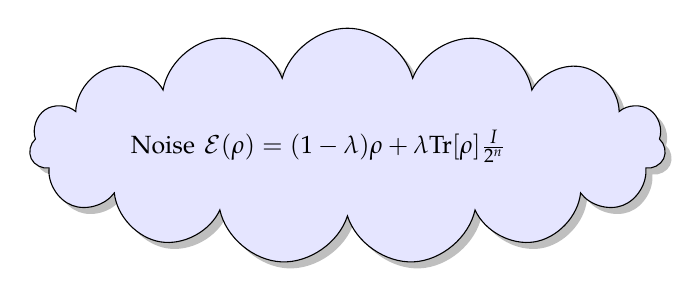
\begin{tikzpicture}
        \node[draw, cloud, cloud puffs=15, cloud ignores aspect,
            minimum width=6cm, minimum height=3cm,
            text width=5.5cm, align=left,
            fill=blue!10, drop shadow]
        {
            \small
            Noise $\mathcal{E}(\rho) = (1 - \lambda) \rho + \lambda \text{Tr}[\rho] \frac{I}{2^n}$
        };
    \end{tikzpicture}
    \scalebox{0.55}{\begin{tikzpicture}[x=1cm, y=-1.3cm,
        every node/.style={transform shape} % Ensures scaling affects nodes correctly
    ]
    % Expand the bounding box to include shadows
    \useasboundingbox (-3,-1) rectangle (15,4); % Adjusted to fit content and shadows
    \begin{scope}[yshift=0.5cm]
        % Communication Row (Single Alice–Bob Interaction)
        \node at (0.5,0) {\Large \textbf{Alice} \alice{}};
        \node at (2.25,0) {\fbox{1}};
        \node at (3,0) {$\rightarrow$};
        \node at (4,0) {\fcolorbox{orange}{white}{$\ket{\psi_{1}}$}};
        \node at (5.5,0) {\mail{}};
        % \node at (7,0) {\fbox{\search{} $\{E_{m}\}$}};
        \node at (8,0) { \search $\{\Pi_{m}\}$};
        % \node at (9,0) {\fbox{\shortstack{1 (correct)\\ 2 (error)}}};
        \node at (11,0) {\Large \textbf{Bob} \bob{}};

        % Sticky Note under Alice
        \node[draw, fill=yellow!30, drop shadow={shadow xshift=3pt, shadow yshift=-3pt},
            text width=5.2cm, rounded corners=4pt, inner sep=10pt, align=left]
        at (0.5,2.0) {
            \begin{minipage}{\linewidth}
                \textbf{Alice’s knowledge}
                \begin{align*}
                    \ket{\psi_{1}}   & = \ket{0}                            \\
                    \ket{\psi_{2}}   & = \frac{\ket{0} + \ket{1}}{\sqrt{2}} \\
                    S_{\text{prior}} & = \{p_1, p_2\} = \{0.5, 0.5\}
                \end{align*}
            \end{minipage}
        };


        % Sticky Note under Bob
        \node[draw, fill=yellow!30, drop shadow={shadow xshift=3pt, shadow yshift=-3pt},
            text width=5.2cm, rounded corners=4pt, inner sep=10pt, align=left]
        at (11,2.0) {
            \begin{minipage}{\linewidth}
                \textbf{Bob’s knowledge}
                \begin{align*}
                    \ket{\psi_{1}}   & = \ket{0}                            \\
                    \ket{\psi_{2}}   & = \frac{\ket{0} + \ket{1}}{\sqrt{2}} \\
                    S_{\text{prior}} & = \{p_1, p_2\} = \{0.5, 0.5\}
                \end{align*}
            \end{minipage}
        };
    \end{scope}
\end{tikzpicture}
}
\end{frame}

\begin{frame}
    \frametitle{Previous work - FRIO}
    Assume that the input quantum states are \textbf{mixed states}
    instead of pure states.\\
    For minimum error discrimination, the formulation is unchanged.\\
    For unambiguous discrimination, it becomes almost impossible to find a
    solution.\\
    \vspace{0.2cm}
    \cite{RN37} Fixed rate of inconclusive outcome (FRIO)\\

    % Depends on {table}{xcolor}
    \begin{table}[ht]
        \begin{tabular}{c | c c c c}
                       & $\Pi_{1}$            & $\Pi_{2}$            & $\Pi_{3}$            & $\Pi_{?}$                      \\
            \hline
            $\rho_{1}$ & \cellcolor{green!20} & \cellcolor{red!20}   & \cellcolor{red!20}   & \cellcolor{yellow!30}          \\
            $\rho_{2}$ & \cellcolor{red!20}   & \cellcolor{green!20} & \cellcolor{red!20}   & \cellcolor{yellow!30}  $\beta$ \\
            $\rho_{3}$ & \cellcolor{red!20}   & \cellcolor{red!20}   & \cellcolor{green!20} & \cellcolor{yellow!30}          \\
        \end{tabular}
        \caption{Probability matrix $p(m,i) = p_{i} \bra{\psi_{i}} \Pi_{m} \ket{\psi_{i}}$}
        % \label{tab:}
    \end{table}
\end{frame}

\begin{frame}
    \frametitle{Semidefinite programming for FRIO}
    % Depends on {table}{xcolor}
    \begin{table}[ht]
        \begin{tabular}{c | c c c c}
                       & $\Pi_{1}$            & $\Pi_{2}$            & $\Pi_{3}$            & $\Pi_{?}$                      \\
            \hline
            $\rho_{1}$ & \cellcolor{green!20} & \cellcolor{red!20}   & \cellcolor{red!20}   & \cellcolor{yellow!30}          \\
            $\rho_{2}$ & \cellcolor{red!20}   & \cellcolor{green!20} & \cellcolor{red!20}   & \cellcolor{yellow!30}  $\beta$ \\
            $\rho_{3}$ & \cellcolor{red!20}   & \cellcolor{red!20}   & \cellcolor{green!20} & \cellcolor{yellow!30}          \\
        \end{tabular}
    \end{table}
    \begin{align}
         & \underset{\{\Pi\}}{\text{maximize}} &  & \raisebox{-0.3em}{\textcolor{green}{\rule{1em}{1em}}} \; P_{D}=\sum_{i=1}^{m} p_{i} \operatorname{Tr}(\rho_{i} \Pi_{i})               \\
         & \text{subject to}                   &  & \Pi_{i} \succeq 0, \quad i = 0, \ldots, m                                                                                             \\
         &                                     &  & \sum_{i=0}^{m} \Pi_i = I                                                                                                              \\
         &                                     &  & \raisebox{-0.3em}{\textcolor{yellow}{\rule{1em}{1em}}} \; P_{inc}=\sum_{i=1}^{m} p_{i} \operatorname{Tr}(\rho_{i} \Pi_{0}) \geq \beta
    \end{align}
\end{frame}

\begin{frame}
    \frametitle{Our problem formulation 1 -- CrossQD}
    Inspired by the type-I error and type-II error in hypothesis testing, we
    derive a new set of constraints.
    \begin{table}[ht]
        \begin{tabular}{c | c c }
                       & $\Pi_{1}$                          & $\Pi_{2}$                            \\
            \hline
            $\rho_{1}$ & \cellcolor{green!20} True positive & \cellcolor{red!20}   False negative  \\
            $\rho_{2}$ & \cellcolor{red!20} False positive  & \cellcolor{green!20}   True negative \\
        \end{tabular}
        \caption{An analogy to the confusion matrix}
    \end{table}
    \begin{table}[ht]
        \begin{tabular}{c | c c c c}
                       & $\Pi_{1}$              & $\Pi_{2}$                 & $\Pi_{3}$               & $\Pi_{?}$             \\
            \hline
            $\rho_{1}$ & \cellcolor{green!20}   & \cellcolor{red!20}    $*$ & \cellcolor{red!20}      & \cellcolor{yellow!30} \\
            $\rho_{2}$ & \cellcolor{red!20} $-$ & \cellcolor{green!20} $+$  & \cellcolor{red!20}  $-$ & \cellcolor{yellow!30} \\
            $\rho_{3}$ & \cellcolor{red!20}     & \cellcolor{red!20}   $*$  & \cellcolor{green!20}    & \cellcolor{yellow!30} \\
        \end{tabular}
    \end{table}
\end{frame}

\begin{frame}
    \frametitle{Semidefinite programming for CrossQD}
    % Depends on {table}{xcolor}
    \begin{table}[ht]
        \begin{tabular}{c | c c c c}
                       & $\Pi_{1}$              & $\Pi_{2}$                 & $\Pi_{3}$               & $\Pi_{?}$             \\
            \hline
            $\rho_{1}$ & \cellcolor{green!20}   & \cellcolor{red!20}    $*$ & \cellcolor{red!20}      & \cellcolor{yellow!30} \\
            $\rho_{2}$ & \cellcolor{red!20} $-$ & \cellcolor{green!20} $+$  & \cellcolor{red!20}  $-$ & \cellcolor{yellow!30} \\
            $\rho_{3}$ & \cellcolor{red!20}     & \cellcolor{red!20}   $*$  & \cellcolor{green!20}    & \cellcolor{yellow!30} \\
        \end{tabular}
    \end{table}
    {
    \scriptsize
    \begin{align}
         & \underset{\{\Pi\}}{\text{maximize}} &            & P_{D}=\sum_{i=1}^{m} p_{i} \operatorname{Tr}(\rho_{i} \Pi_{i})                                                                                                      \\
         & \text{subject to}                   &            & \Pi_{i} \succeq 0, \quad i = 0, \ldots, m                                                                                                                           \\
         &                                     &            & \sum_{i=0}^{m} \Pi_i = I                                                                                                                                            \\
         &                                     & - \;\;\;\; & P(O_i \mid \rho_i) = \frac{p_i \, \operatorname{Tr}(\rho_i \Pi_i)}{\sum_{j=1}^{m} p_i \, \operatorname{Tr}(\rho_i \Pi_j)} \geq 1 - \alpha_i, \quad i = 1, \ldots, m \\
         &                                     & * \;\;\;\; & P(\rho_i \mid O_i) = \frac{p_i \, \operatorname{Tr}(\rho_i \Pi_i)}{\sum_{j=1}^{m} p_j \, \operatorname{Tr}(\rho_j \Pi_i)} \geq 1 - \beta_i, \quad i = 1, \ldots, m
    \end{align}
    }
\end{frame}

\begin{frame}
    \frametitle{Benefits of CrossQD}
    \begin{itemize}
        \item We can make sure the resulting POVM keeps the states we want.
        \item We have more flexibility to tweak the POVM than with FRIO.
              % \item We didn't really know if there are other benefits.
    \end{itemize}
\end{frame}

% \begin{frame}
%     \frametitle{Observations of CrossQD results}
%     
% \end{frame}

\begin{frame}
    \frametitle{Problem formulation 2 -- FitQD}
    Goal: Find a POVM such that the resulting probability distribution is the
    same as the ideal distribution $\pi$, generated by OP-UQSD.\\
    Question: What does the "distribution" mean here?
    \begin{table}[ht]
        \begin{tabular}{c | c | c | c | c | c}
                          & $\Pi_{1}$            & $\Pi_{2}$            & $\Pi_{3}$            & $\Pi_{4} = \Pi_{?}$   \\
            \hline
            $\rho_{1}$    & \cellcolor{green!20} & \cellcolor{red!20}   & \cellcolor{red!20}   & \cellcolor{yellow!30} \\
            $\rho_{2}$    & \cellcolor{red!20}   & \cellcolor{green!20} & \cellcolor{red!20}   & \cellcolor{yellow!30} \\
            $\rho_{3}$    & \cellcolor{red!20}   & \cellcolor{red!20}   & \cellcolor{green!20} & \cellcolor{yellow!30} \\
            \hline
            sum of column & $\mu_{1}$            & $\mu_{2}$            & $\mu_{3}$            & $\mu_{4}$             \\
            OP-UQSD       & $\pi_{1}$            & $\pi_{2}$            & $\pi_{3}$            & $\pi_{4}$
        \end{tabular}
        \caption{Our definition of the distribution that we want to approach}
    \end{table}
\end{frame}

\begin{frame}
    \frametitle{Semidefinite programming for FitQD}
    % Depends on {table}{xcolor}
    \begin{table}[ht]
        \begin{tabular}{c | c | c | c | c | c}
                          & $\Pi_{1}$            & $\Pi_{2}$            & $\Pi_{3}$            & $\Pi_{4} = \Pi_{?}$   \\
            \hline
            $\rho_{1}$    & \cellcolor{green!20} & \cellcolor{red!20}   & \cellcolor{red!20}   & \cellcolor{yellow!30} \\
            $\rho_{2}$    & \cellcolor{red!20}   & \cellcolor{green!20} & \cellcolor{red!20}   & \cellcolor{yellow!30} \\
            $\rho_{3}$    & \cellcolor{red!20}   & \cellcolor{red!20}   & \cellcolor{green!20} & \cellcolor{yellow!30} \\
            \hline
            sum of column & $\mu_{1}$            & $\mu_{2}$            & $\mu_{3}$            & $\mu_{4}$             \\
            OP-UQSD       & $\pi_{1}$            & $\pi_{2}$            & $\pi_{3}$            & $\pi_{4}$
        \end{tabular}
    \end{table}
    {
    \scriptsize
    \begin{align}
         & \underset{\{\Pi\}}{\text{maximize}} &  & P_{D}=\sum_{i=1}^{m} p_{i} \operatorname{Tr}(\rho_{i} \Pi_{i})                                      \\
         & \text{subject to}                   &  & \Pi_{i} \succeq 0, \quad i = 0, \ldots, m                                                           \\
         &                                     &  & \sum_{i=0}^{m} \Pi_i = I                                                                            \\
         &                                     &  & \mu_{i} = \sum_{j=1}^{m} p_j \, \operatorname{Tr}(\rho_j \Pi_i) = \pi_{i}, \quad i = 1, \ldots, m+1
    \end{align}
    }
\end{frame}

\begin{frame}
    \frametitle{Some other attempts}
    We have tried several approaches before we came up with FitQD.
    \begin{enumerate}
        \item Use the POVM from OP-UQSD
        \item Gradient descent/Bayesian optimization as outer-loop, solving SDP as inner-loop (a mess)
    \end{enumerate}
    
    \vspace{0.1cm}
    \centering
    \scalebox{0.4}{\usetikzlibrary{shapes.geometric, arrows}

\tikzstyle{startstop} = [rectangle, rounded corners,
minimum width=3cm,
minimum height=1cm,
text centered,
text width=3cm,
draw=black,
fill=red!30]

\tikzstyle{io} = [trapezium,
trapezium stretches=true, % A later addition
trapezium left angle=70,
trapezium right angle=110,
minimum width=3cm,
minimum height=1cm,
align=center,
text width=5cm,
text centered,
draw=black, fill=blue!30]

\tikzstyle{process} = [rectangle,
minimum width=3cm,
minimum height=1cm,
text centered,
text width=4cm,
draw=black,
fill=orange!30]

\tikzstyle{decision} = [diamond,
minimum width=3cm,
minimum height=1cm,
text width=4cm,
aspect=2,
inner sep=-1ex,
text centered,
draw=black,
fill=green!30]
\tikzstyle{arrow} = [thick,->,>=stealth]

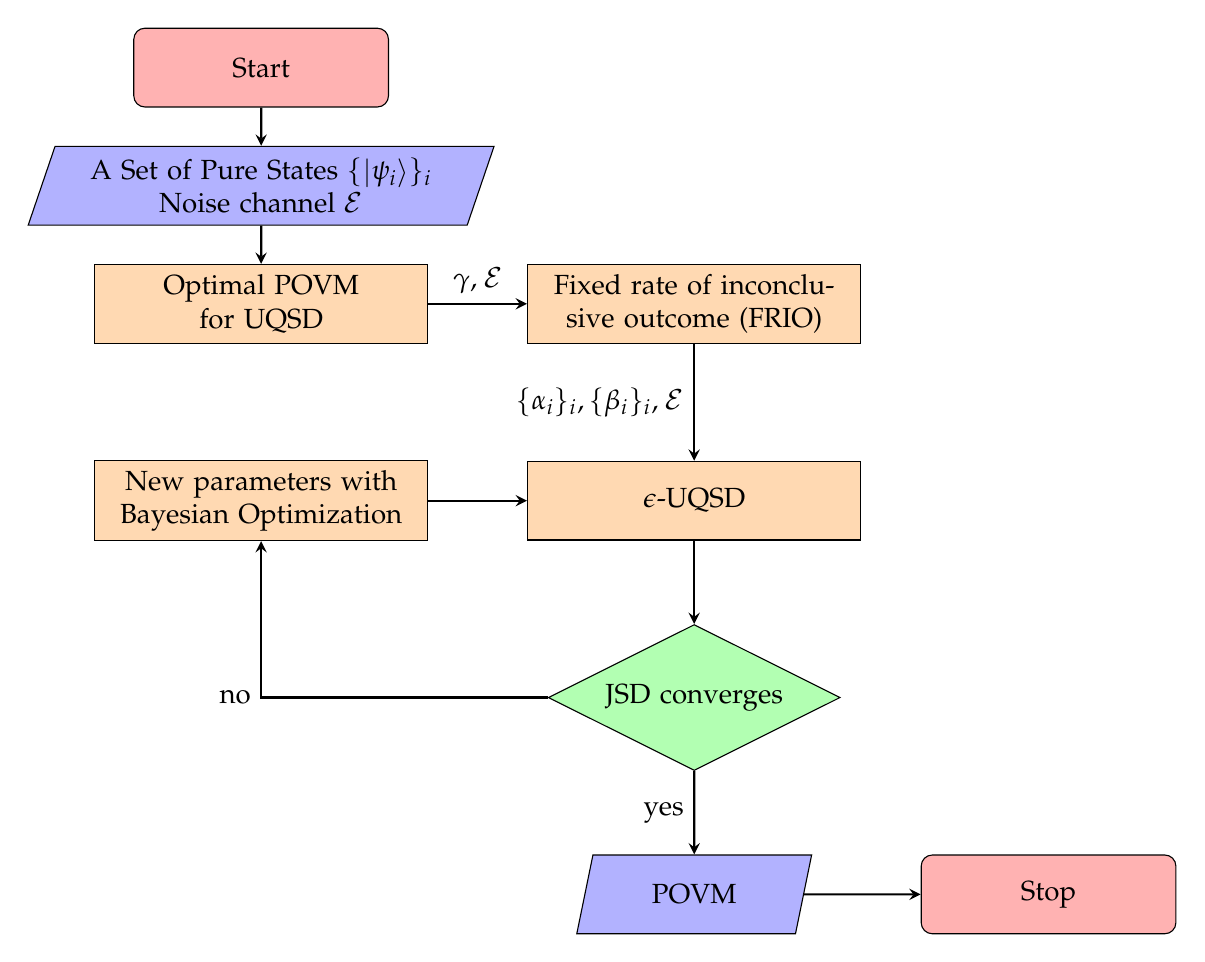
\begin{tikzpicture}[node distance=1.5cm]

    \node (start) [startstop] {Start};
    \node (in1) [io, below of=start] {%
        A Set of Pure States $\{\ket{\psi_{i}}\}_{i}$\\
        Noise channel $\mathcal{E}$\\
    };

    \node (pro1) [process, below of=in1] {
        Optimal POVM for UQSD\\
    };

    \node (pro2) [process, right of=pro1, xshift=4cm] {
        Fixed rate of inconclusive outcome (FRIO)\\
    };

    \node (pro3) [process, below of=pro2, yshift=-1cm] {
        $\epsilon$-UQSD\\
    };
    \node (pro4) [process, left of=pro3, xshift=-4cm] {
        New parameters with\\
        Bayesian Optimization\\
    };

    \node (dec1) [decision, below of=pro3, yshift=-1cm] {JSD converges};
    \node (out1) [io, below of=dec1, yshift=-1cm, text width=2cm] {
        POVM
    };
    \node (stop) [startstop, right of=out1, xshift=3cm] {Stop};

    \draw [arrow] (start) -- (in1);
    \draw [arrow] (in1) -- (pro1);
    \draw [arrow] (pro1) -- node[anchor=south] {$\gamma$, $\mathcal{E}$} (pro2);
    \draw [arrow] (pro2) -- node[anchor=east] {$\{\alpha_{i}\}_{i}, \{\beta_{i}\}_{i}$, $\mathcal{E}$} (pro3);
    \draw [arrow] (pro3) -- (dec1);
    % \draw [arrow] (dec1) -- ++(-3,0) node[left] {no} |- (pro3.west);
    \draw [arrow] (dec1) -| node[left] {no} (pro4);
    \draw [arrow] (pro4) -- (pro3);
    \draw [arrow] (dec1) -- node[anchor=east] {yes} (out1);
    \draw [arrow] (out1) -- (stop);

\end{tikzpicture}}
    % Define distance and gradient descent
\end{frame}

\begin{frame}
    \begin{table}[htbp]
        \frametitle{Comparison of our attempts}
        simple\_2 is the set of states mentioned in Frame \ref{frame:nonortho_ex}.
        \vspace*{0.1cm}
        
        \centering
        \scalebox{0.6}{
            \begin{tabular}{c|ccccc}
                \toprule
                Dep. noise level & \makecell{ideal optimal}      & \makecell{FRIO                                                       \\ (ideal pinc)} & \makecell{crossQD\\ (0.75*noise)} & \makecell{crossQD-2\\ (ideal params, ideal pinc)} & \makecell{FitQD\\ (ideal distrib)} \\
                \midrule
                1.00E-06         & \cellcolor{green!20} 0.000000 & 0.002606       & 0.001185 & 0.000003 & \cellcolor{green!20} 0.000000 \\
                3.16E-05         & \cellcolor{green!20} 0.000000 & 0.002605       & 0.002086 & 0.000003 & \cellcolor{green!20} 0.000000 \\
                1.00E-05         & 0.000002                      & 0.002601       & 0.003583 & 0.000006 & \cellcolor{green!20} 0.000000 \\
                3.16E-04         & 0.000005                      & 0.002558       & 0.006124 & 0.000054 & \cellcolor{green!20} 0.000000 \\
                1.00E-04         & 0.000015                      & 0.002120       & 0.009940 & 0.000202 & \cellcolor{green!20} 0.000000 \\
                3.16E-03         & 0.000049                      & 0.000022       & 0.015885 & 0.000044 & \cellcolor{green!20} 0.000000 \\
                1.00E-03         & 0.000154                      & 0.000068       & 0.023398 & 0.000073 & \cellcolor{green!20} 0.000000 \\
                3.16E-02         & 0.000487                      & 0.000247       & 0.034139 & 0.000094 & \cellcolor{green!20} 0.000000 \\
                1.00E-02         & 0.001538                      & 0.001412       & 0.054889 & 0.000263 & \cellcolor{green!20} 0.000000 \\
                3.16E-01         & 0.004845                      & 0.002258       & 0.105572 & 0.001372 & \cellcolor{green!20} 0.000000 \\
                1.00E-01         & 0.015152                      & 0.007085       & 0.226254 & 0.005255 & \cellcolor{green!20} 0.000000 \\
                \bottomrule
            \end{tabular}
        }
        \caption{Jensen-Shannon distance comparison (The lower the better) for \texttt{simple\_2} under different noise levels.}
    \end{table}
\end{frame}

\begin{frame}[label=frame3]
    \frametitle{Comparison of different formulations}
    \begin{table}[ht]
        \begin{tabular}{c | c c | c c}
                               & OP-UQSD    & FRIO       & CrossQD    & FitQD      \\
            \hline
            Our proposal       &            &            & \checkmark & \checkmark \\
            Max $P_{succ}$     & \checkmark & \checkmark & \checkmark & \checkmark \\
            Noise aware        &            & \checkmark & \checkmark & \checkmark \\
            Confidence aware   &            &            & \checkmark &            \\
            Distribution aware & -          &            &            & \checkmark \\
        \end{tabular}
        \caption{Comparison of different formulations}
    \end{table}
\end{frame}


\section{Quantum Circuit Synthesis for QSD}

\begin{frame}
    \frametitle{Synthesis flow}
    \centering
    \scalebox{0.45}{
        \usetikzlibrary{shapes.geometric, arrows.meta, positioning}

% TODO Remove random properties
% Proper definition of input POVM
\tikzstyle{startstop} = [rectangle, rounded corners,
minimum width=3cm,
minimum height=1cm,
text centered,
text width=3cm,
draw=black,
fill=red!30]

\tikzstyle{io} = [trapezium,
trapezium stretches=true, % A later addition
trapezium left angle=70,
trapezium right angle=110,
minimum width=3cm,
minimum height=1cm,
align=center,
text width=5cm,
text centered,
draw=black, fill=blue!30]

\tikzstyle{process} = [rectangle,
minimum width=3cm,
minimum height=1cm,
text centered,
text width=4cm,
draw=black,
fill=orange!30]

\tikzstyle{decision} = [diamond,
minimum width=3cm,
minimum height=1cm,
text width=4cm,
aspect=2,
inner sep=-1ex,
text centered,
draw=black,
fill=green!30]
\tikzstyle{arrow} = [thick,->,>=stealth]

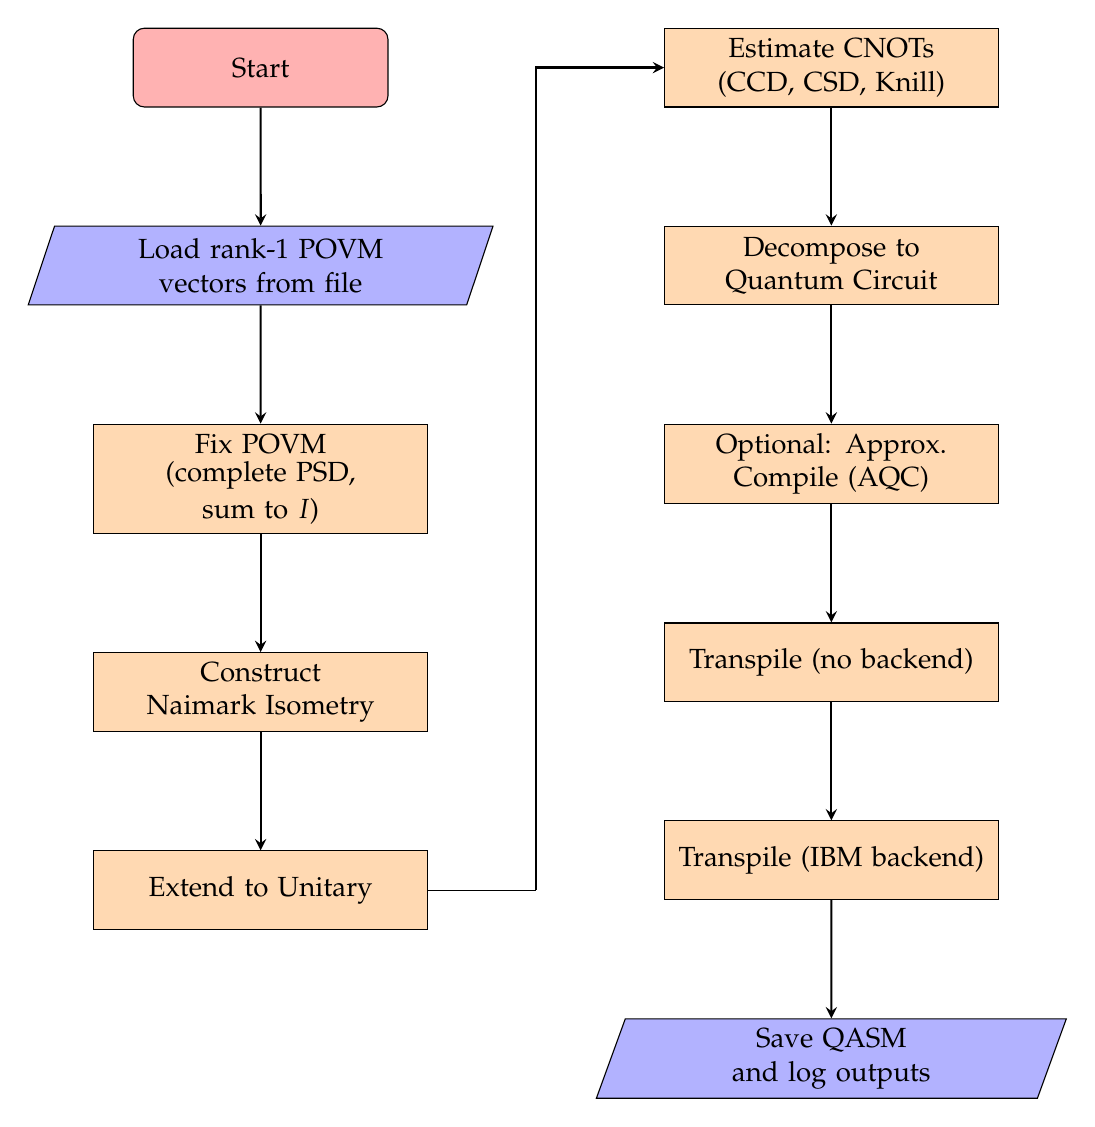
\begin{tikzpicture}[node distance=1.5cm and 0.5cm]

    \node (start) [startstop] {Start};
    % \node (input) [io, below=of start] {User input: \texttt{nq}, \texttt{ns}, \texttt{seed}, \texttt{tag}};
    \node (load) [io, below=of start] {Load rank-1 POVM vectors from file};
    % \node (load) [process, below=of input] {Load rank-1 POVM vectors from file};
    \node (fix) [process, below=of load] {\shortstack{Fix POVM \\(complete PSD, \\sum to $I$)}};
    \node (iso) [process, below=of fix] {Construct Naimark Isometry};
    \node (extend) [process, below=of iso] {Extend to Unitary};
    \coordinate (pt) at ($(extend) + (3.5, 0)$);
    \node (est) [process, right=of start, xshift=3cm] {Estimate CNOTs (CCD, CSD, Knill)};
    \node (synth) [process, below=of est] {Decompose to Quantum Circuit};
    \node (approx) [process, below=of synth] {Optional: Approx. Compile (AQC)};
    \node (transpile1) [process, below=of approx] {Transpile (no backend)};
    \node (transpile2) [process, below=of transpile1] {Transpile (IBM backend)};
    \node (save) [io, below=of transpile2] {\shortstack{Save QASM \\ and log outputs}};

    % \draw [arrow] (start) -- (input);
    % \draw [arrow] (input) -- (load);
    \draw [arrow] (start) -- (load);
    \draw [arrow] (load) -- (fix);
    \draw [arrow] (fix) -- (iso);
    \draw [arrow] (iso) -- (extend);
    \draw (extend) -- (pt);
    \draw [arrow] (pt) |- (est);
    \draw [arrow] (est) -- (synth);
    \draw [arrow] (synth) -- (approx);
    \draw [arrow] (approx) -- (transpile1);
    \draw [arrow] (transpile1) -- (transpile2);
    \draw [arrow] (transpile2) -- (save);

\end{tikzpicture}

    }
\end{frame}

\begin{frame}
    \frametitle{Naimark's dilation theorem (1/5)}
    Naimark's dilation theorem shows how POVMs can be obtained from PVMs
    acting on a larger space. (Refer to Frame \ref{frame:povm})

    \begin{theorem}[Naimark's dilation theorem]
        If ${\displaystyle \{F_{i}\}_{i=1}^{n}}$ is a POVM acting on a Hilbert space
        ${\mathcal {H}}_{A}$ of dimension $d_{A}$, then there exists a PVM
        $\{\Pi _{i}\}_{i=1}^{n}$ acting on a Hilbert space
        ${\mathcal {H}}_{A'}$ of dimension
        $d_{A'}$ and an isometry
        $V:{\mathcal {H}}_{A}\to {\mathcal {H}}_{A'}$ such that for all $i$,
        $F_{i}=V^{\dagger }\Pi _{i}V.$
    \end{theorem}

    \begin{center}
        \scalebox{0.6}{
            \begin{quantikz}[column sep=0.5cm, row sep=0.4cm]
    & \lstick[3]{$\ket{\psi_1}$} & \qw & \gate[3]{\textsf{POVM}} & \qw \\
    & & \qw & \qw  & \qw                     \\
    & & \qw & \qw  & \qw                     \\
\end{quantikz}
\hspace{0.5cm}
$\equiv$
\begin{quantikz}[column sep=0.5cm, row sep=0.4cm]
    & \lstick[3]{$\ket{\psi_1}$} & \qw & \gate[5]{\textsf{PVM}} & \qw \\
    & & \qw & & \qw                     \\
    & & \qw & & \qw                     \\
    & \lstick[2]{$\ket{\psi_{anc}}$}      & \qw & \qw      & \qw            \\
    &      & \qw & \qw    & \qw          \\
\end{quantikz}
        }
    \end{center}
\end{frame}

\begin{frame}
    \frametitle{Naimark's dilation theorem (2/5)}
    \begin{theorem}[Naimark's dilation theorem]
        If ${\displaystyle \{F_{i}\}_{i=1}^{n}}$ is a POVM acting on a Hilbert space
        ${\displaystyle {\mathcal {H}}_{A}}$ of dimension
        ${\displaystyle d_{A}}$, then there exists a PVM
        ${\displaystyle \{\Pi _{i}\}_{i=1}^{n}}$ acting on a Hilbert space
        ${\displaystyle {\mathcal {H}}_{A'}}$ of dimension
        ${\displaystyle d_{A'}}$ and an isometry
        ${\displaystyle V:{\mathcal {H}}_{A}\to {\mathcal {H}}_{A'}}$ such that for all $i$,
        ${\displaystyle F_{i}=V^{\dagger }\Pi _{i}V.}$
    \end{theorem}
    For the particular case of a \textbf{rank-1 POVM}, i.e., when
    ${\displaystyle F_{i}=|f_{i}\rangle \langle f_{i}|}$ for some (unnormalized) vectors
    ${\displaystyle |f_{i}\rangle }$, this isometry can be constructed as
    \begin{align}
        V = \Sigma_{i=1}^{n} \ket{i}_{A'}\bra{f_{i}}_{A}
    \end{align}
    and the PVM is given simply by
    ${\displaystyle \Pi _{i}=|i\rangle \langle i|_{A'}}$. Note that here
    ${\displaystyle d_{A'}=n}$.
\end{frame}

\begin{frame}
    \frametitle{Naimark's dilation theorem (3/5)}
    \begin{theorem}[Naimark's dilation theorem]
        If ${\displaystyle \{F_{i}\}_{i=1}^{n}}$ is a POVM acting on a Hilbert space
        ${\displaystyle {\mathcal {H}}_{A}}$ of dimension
        ${\displaystyle d_{A}}$, then there exists a PVM
        ${\displaystyle \{\Pi _{i}\}_{i=1}^{n}}$ acting on a Hilbert space
        ${\displaystyle {\mathcal {H}}_{A'}}$ of dimension
        ${\displaystyle d_{A'}}$ and an isometry
        ${\displaystyle V:{\mathcal {H}}_{A}\to {\mathcal {H}}_{A'}}$ such that for all $i$,
        ${\displaystyle F_{i}=V^{\dagger }\Pi _{i}V.}$
    \end{theorem}
    In the general case, the isometry and PVM can be constructed by defining
    ${\displaystyle {\mathcal {H}}_{A'}={\mathcal {H}}_{A}\otimes {\mathcal {H}}_{B}}$,
    ${\displaystyle \Pi _{i}=\operatorname {I} _{A}\otimes |i\rangle \langle i|_{B}}$, and
    ${\displaystyle V=\sum _{i=1}^{n}{\sqrt {F_{i}}}_{A}\otimes {|i\rangle }_{B}.}$
    Note that here
    ${\displaystyle d_{A'}=nd_{A}}$, so this is a more wasteful construction.
\end{frame}

\begin{frame}
    \frametitle{Naimark's dilation theorem (4/5)}
    \begin{itemize}
        \item \textbf{The probability is transformation-invariant}\\
              In either case, the probability of obtaining outcome
              $i$ with this PVM, and the state suitably transformed by the isometry, is the same as the probability of obtaining it with the original POVM:
              ${\displaystyle {\text{Prob}}(i)=\operatorname {tr} \left(V\rho _{A}V^{\dagger }\Pi _{i}\right)=\operatorname {tr} \left(\rho _{A}V^{\dagger }\Pi _{i}V\right)=\operatorname {tr} (\rho _{A}F_{i})}$
        \item \textbf{A recipe for a physical realisation of the POVM}\\
              We can always do it by extending the isometry
              $V$ into a unitary $U$, that is, finding
              $U$ such that ${\displaystyle V|i\rangle _{A}=U|i\rangle _{A'}}$
              for $i$ from 1 to $d_{A}$.
        \item \textbf{In other words}\\
              The recipe for realizing the POVM described by
              $\{F_{i}\}_{i=1}^{n}$ on a quantum state $\rho$
              is then to embed the quantum state in the Hilbert space
              ${\mathcal {H}}_{A'}$, evolve it with the unitary
              $U$, and make the projective measurement described by the PVM
              ${\displaystyle \{\Pi _{i}\}_{i=1}^{n}}$.
    \end{itemize}
\end{frame}

\begin{frame}
    \frametitle{Naimark's dilation theorem (5/5)}
    \centering
    \tikzexternaldisable
    \scalebox{0.45}{
        \input{../figures/naimark_flow.tex}
    }
    \tikzexternalenable
    % \caption{Our flow to apply Naimark's theorem to a POVM}

    For each POVM element, first use SVD to decompose the
\end{frame}

\begin{frame}
    \frametitle{Make sure every element is rank-1}
    \begin{itemize}
        \item Usually the POVM element representing the inconclusive result
              is not rank-1, so we have to decompose it.
        \item For such element $\Pi_{m}$, we use singular value decomposition
              (SVD) to find rank-1 vectors $\ket{\phi}$.
              \begin{align}
                   & \Pi_{m} = U \Sigma V^{T}                           \\
                   & \Pi_{m} = \Sigma_{i} \ket{\phi_{i}} \bra{\phi_{i}} \\
                   & \ket{\phi_{i}} = U_{i} \times s_{i}.
              \end{align}
    \end{itemize}
\end{frame}

\begin{frame}
    \frametitle{Quantum circuits for isometries}
    \cite{RN12}\\
    Both Qiskit and qclib (\cite{qclib}) implemented the three decomposition
    algorithms (knill, ccd, and csd) introduced in this work.\\
    Since the size of the considered quantum states are relatively small (2 to 5 qubits),
    the scalability of these algorithms (noticeable for $\# qubits >= 8$)
    does not affect our results.\\
    The intuition is to estimate CNOTs of the three algorithms, then
    synthesize with the algorithm with the fewest CNOTs.
\end{frame}

\begin{frame}
    \frametitle{Example - three coherent states}
    \begin{figure}[htbp]
    \centering

    \begin{subfigure}[b]{0.23\textwidth}
        \centering
        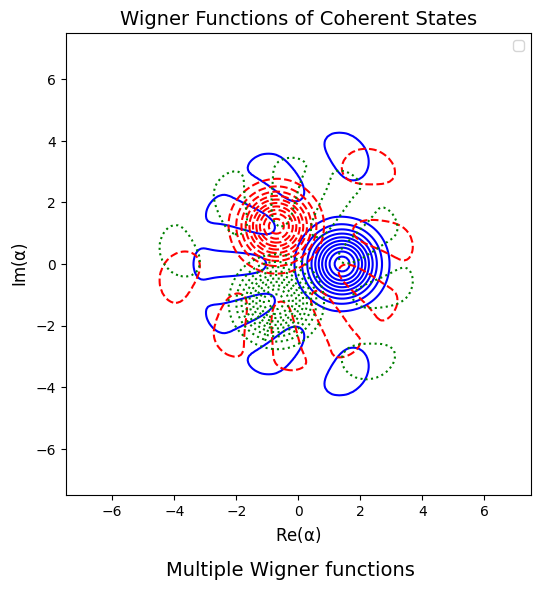
\includegraphics[width=\linewidth]{figures/q3_n3.png}
        \caption{\#qubits = 3}
        \label{fig:coh_q3_n3}
    \end{subfigure}
    \hfill
    \begin{subfigure}[b]{0.23\textwidth}
        \centering
        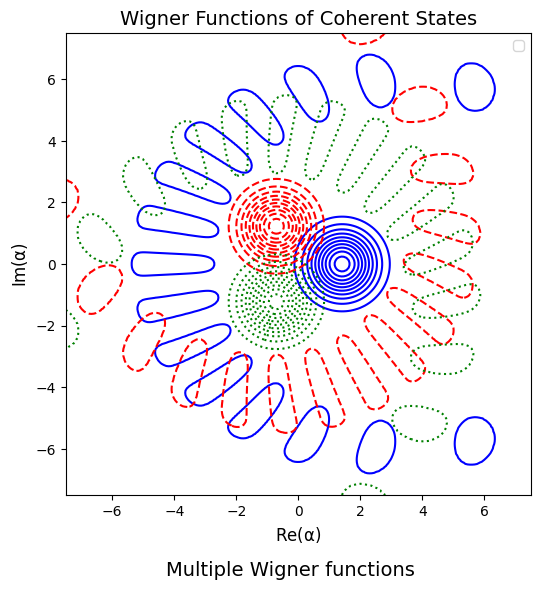
\includegraphics[width=\linewidth]{figures/q4_n3.png}
        \caption{\#qubits = 4}
        \label{fig:coh_q4_n3}
    \end{subfigure}
    \hfill
    \begin{subfigure}[b]{0.23\textwidth}
        \centering
        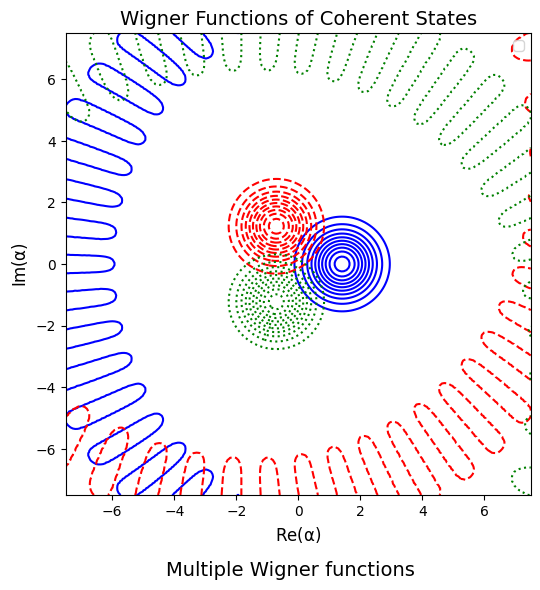
\includegraphics[width=\linewidth]{figures/q5_n3.png}
        \caption{\#qubits = 5}
        \label{fig:coh_q5_n3}
    \end{subfigure}
    \hfill
    \begin{subfigure}[b]{0.23\textwidth}
        \centering
        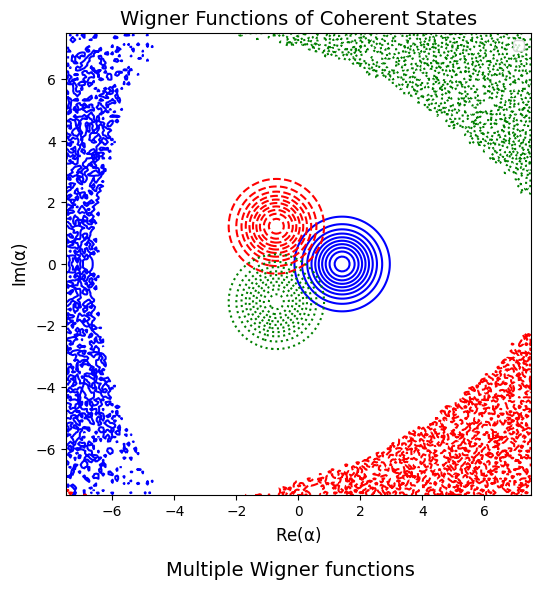
\includegraphics[width=\linewidth]{figures/q6_n3.png}
        \caption{\#qubits = 6}
        \label{fig:coh_q6_n3}
    \end{subfigure}

    \caption{Wigner functions for multiple truncated coherent states with
        different number of qubits. Blue, green, red represent the state
        $\ket{\alpha}$ with
        $\alpha = 0, e^{\frac{2\pi}{3} j}, e^{\frac{4\pi}{3} j}$, respectively.}
    \label{fig:coh_comparison}
\end{figure}
\end{frame}

\begin{frame}
    \frametitle{Results - three coherent states}

    % I copied the whole ../figures/synth_coh_table.tex since the table
    % requires to be scaled down a bit.
    \begin{table}[htbp]
        \centering
        \caption{Comparison of quantum circuit synthesis methods for
            discriminating three
            coherent states. Here 2Q means the number of two-qubit gates, which is
            also the number of CNOT gates in this case.
            Fidelity is rounded down to the fifth digit.}
        \label{tab:synth_comparison}
        \scalebox{0.42}{
            \renewcommand{\arraystretch}{1.2}
            \begin{tabular}{|c|c||rr||rrr|rrr|rrr|rrr|}
                \hline
                \textbf{\# Qubits}
                  & \multicolumn{1}{c||}{\textbf{Fidelity}}
                  & \multicolumn{2}{c||}{\textbf{Original}}
                  & \multicolumn{3}{c|}{\textbf{Resynthesis}}
                  & \multicolumn{3}{c|}{\textbf{Approx\_deg = 1.00}}
                  & \multicolumn{3}{c|}{\textbf{Approx\_deg = 0.97}}
                  & \multicolumn{3}{c|}{\shortstack{\textbf{AQC (2Q = 10)}}}                                                                                                                       \\
                  &                                                          & Depth & 2Q    & Depth & 2Q   & Fidelity & Depth & 2Q   & Fidelity & Depth & 2Q   & Fidelity & Depth & 2Q & Fidelity \\
                \hline
                2 & 0.97803                                                  & 84    & 41    & 45    & 20   & 1.00000  & 29    & 14   & 0.99999  & 29    & 14   & 0.59409  & 21    & 10 & 0.35564  \\
                3 & 0.99998                                                  & 430   & 218   & 225   & 100  & 0.99999  & 83    & 61   & 0.99992  & 83    & 61   & 0.88925  & 15    & 10 & 0.96252  \\
                4 & 0.99999                                                  & 2034  & 1025  & 1009  & 444  & 0.99999  & 253   & 252  & 0.99989  & 253   & 252  & 0.13754  & 11    & 10 & 0.32505  \\
                5 & 0.99999                                                  & 8916  & 4474  & 4273  & 1868 & 0.99999  & 817   & 1020 & 0.99990  & 817   & 1020 & 0.00032  & 9     & 10 & 0.25978  \\
                6 & 0.99999                                                  & 37220 & 18634 & 17585 & 7660 & 0.99999  & 2729  & 4091 & 0.99984  & -     & -    & -        & -     & -  & -        \\
                \hline
            \end{tabular}
        }
    \end{table}
\end{frame}

\begin{frame}
    \frametitle{Simulation - three coherent states}
    \begin{itemize}
        \item \textbf{Design under test (DUT)}\\
              One of the predefined pure state $\ket{\psi}$ + the quantum circuit we design
        \item \textbf{Environment}\\
              Increasing depolarizing noise
        \item \textbf{What to observe}\\
              \begin{itemize}
                  \item Outcome distribution from fixed number of shots
                  \item Probabilities from simulated state vector
              \end{itemize}
    \end{itemize}
    We are also curious about
    how noise will affect the discrimination results, and we want to see if smaller circuits work
    well enough for the states using more qubits. We expect the circuits with high process
    fidelity to run successfully, so we will show the results together with noisy simulation.
\end{frame}

\begin{frame}
    \frametitle{David versus Goliath: 4-qubit circuit discriminating a 6-qubit state}
    \begin{itemize}
        \item sv\_coh\_symm\_small(num\_qubits=6)
        \item qc\_iso\_coh\_q3\_n3\_no\_backend\_resynth.qasm
        \item OrderedDict({'u': 208, 'cx': 100})
        \item Depth: 225
    \end{itemize}
    \centering
    \includegraphics[width=0.7\textwidth]{../figures/6_qubit_state_4_qubit_circuit_coh_symm.png}
\end{frame}

\begin{frame}
    \frametitle{Ideal simulation}
    \begin{table}[htbp]
        \centering
        \caption{Simulation results: top measurement outcomes and probabilities}
        \begin{tabular}{c|c|c|c}
            \textbf{Initial State} & \textbf{Top Outcome(s)} & \textbf{Counts} & \textbf{Probabilities} \\
            \hline
            $\ket{\psi_0}$         & \cellcolor{green!20} 000000                  & 585             & 0.5583                 \\
                                   & \cellcolor{yellow!20} 001000                  & 261             & 0.2445                 \\
                                   & \cellcolor{yellow!20} 001001                  & 178             & 0.1971                 \\
            \hline
            $\ket{\psi_1}$         & \cellcolor{green!20} 000001                  & 591             & 0.5624                 \\
                                   & \cellcolor{yellow!20} 001000                  & 257             & 0.2416                 \\
                                   & \cellcolor{yellow!20} 001001                  & 176             & 0.1960                 \\
            \hline
            $\ket{\psi_2}$         & \cellcolor{green!20} 000010                  & 591             & 0.5627                 \\
                                   & \cellcolor{yellow!20} 001000                  & 257             & 0.2416                 \\
                                   & \cellcolor{yellow!20} 001001                  & 176             & 0.1957                 \\
        \end{tabular}
    \end{table}
\end{frame}

\begin{frame}
    \frametitle{Simulation with two-qubit depolarizing noise}
    \centering
    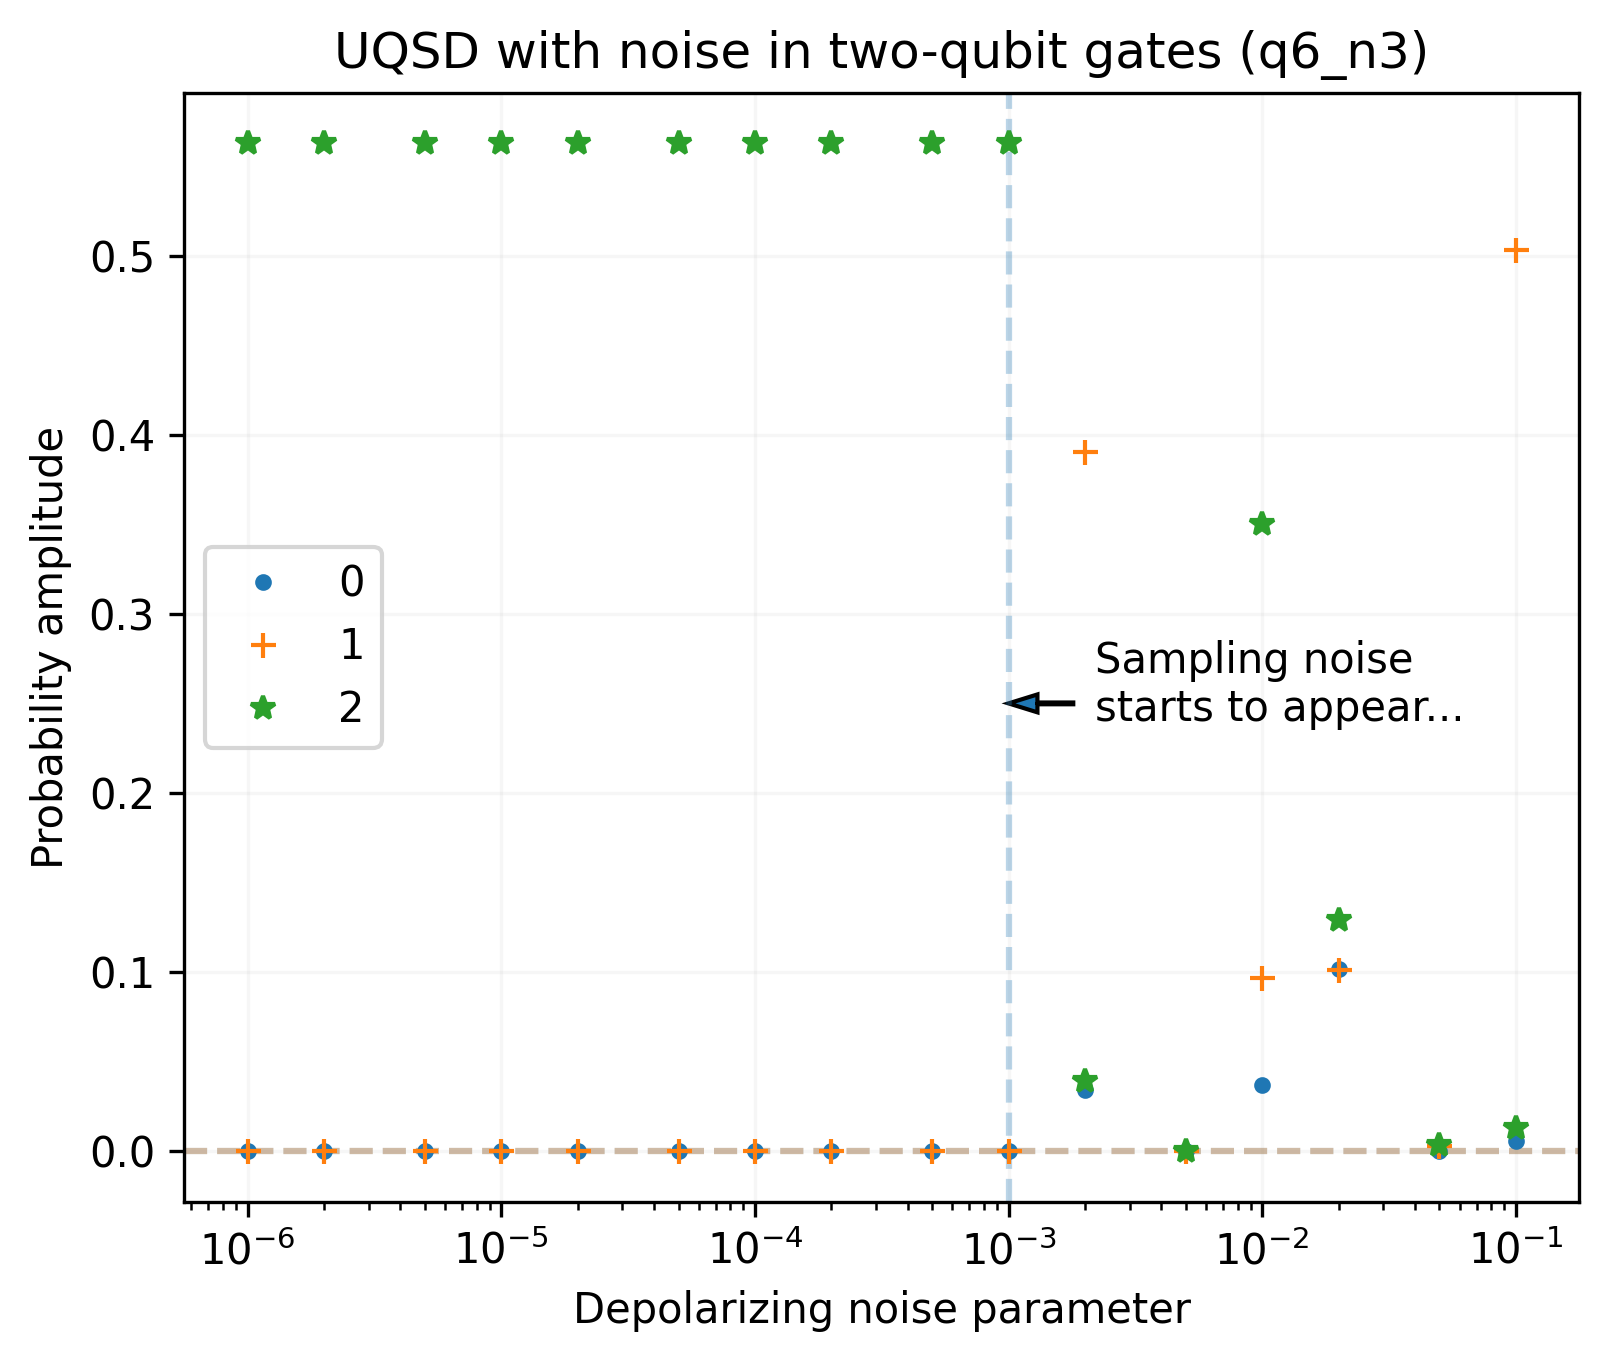
\includegraphics[width=0.7\textwidth]{6q_4circ.png}
\end{frame}
\section{Summary}

\begin{frame}
    \frametitle{Summary}
    \begin{itemize}
        \item We have developed a tool to synthesize and test quantum circuits
              by specifying a quantum state discrimination problem.
        \item We have investigated different formulations of quantum state
              discrimination with mixed states and the result probability
              distribution in mind.
    \end{itemize}
\end{frame}

\section{Appendix}

\subsection{Coherent states}

\begin{frame}
    \frametitle{Related works}
    \cite{RN382}\\
    This work performed a physical experiment for UQSD for 4 coherent states.

\end{frame}

\begin{frame}
    \frametitle{Canonical Coherent States}
    The canonical coherent states have three properties that are mutually equivalent.
    \begin{itemize}
        \item They are eigenvectors of the annihilation operator: $\hat{a}\ket{\alpha}=\alpha\ket{\alpha}$
        \item They are obtained from the vacuum by application of a unitary displacement operator:
              $\ket{\alpha}=(e^{\alpha \hat{a}^{\dagger} - \alpha^{*}\hat{a}})\ket{0}=D(\alpha)\ket{0}$
        \item They are states of minimal uncertainty: $\Delta{X} = \Delta{P} = \sqrt{\frac{\hbar}{2}}$
    \end{itemize}
\end{frame}

\begin{frame}
    \frametitle{Example - State Selection}
    \begin{itemize}
        \item Truncated coherent states and fidelity is important...
              We chose the following three sets of coherent states to demonstrate the dynamics of
              the different methods to search for a proper POVM for state discrimination.
        \item First, we want the set of coherent states to show some symmetric property.
              Since each coherent state correspond to an annihilation operator with a unique eigenvalue,
              we set the eigenvalues to have the same magnitude but different angles and the difference of
              each pair of angles is the same. We can visualize the states with Wigner function, as the figure below.
    \end{itemize}
\end{frame}

\begin{frame}
    \frametitle{Influence of Truncation of Coherent States}
    \begin{center}
        \scalebox{0.17}{
            \includegraphics{../figures/trun_coh.png}
        }
    \end{center}
\end{frame}

\begin{frame}
    \frametitle{Influence of Truncation of Coherent States}
    \begin{itemize}
        \item We also calculated the fidelity of truncated
              coherent states by padding zeros to the same dimension.
        \item A truncated coherent state with the largest dimension
              is selected as the reference.
        \item So for $\alpha = 4$, we will select $N = 64$.
    \end{itemize}
    \begin{table}[ht]
        \centering
        \scalebox{0.55}{
            \begin{tabular}{r r}
                \hline
                \textbf{Fock States (N)} & \textbf{Fidelity}    \\
                \hline
                2                        & 1.525e-06            \\
                4                        & 5.193e-07            \\
                8                        & 2.606e-04            \\
                16                       & 2.674e-01            \\
                32                       & 0.999594             \\  % ← This is the special one
                64                       & 1.0 (0 to 13 digits) \\
                128                      & 1.0 (0 to 13 digits) \\
                256                      & 1.0 (0 to 13 digits) \\
                512                      & 1.0 (0 to 13 digits) \\
                1024                     & 1.0 (0 to 13 digits) \\
                \hline
            \end{tabular}
        }
        \caption{Fidelity of $\ket{\alpha}$ w.r.t N = 1024 ($\alpha = 4$)}
        \label{tab:fock-fidelity}
    \end{table}
\end{frame}

\begin{frame}
    \frametitle{Selecting $\alpha$}
    \begin{itemize}
        \item It is also important to choose $\alpha$ (The eigenvalue of the
              annihilation operator).
        \item Since we know the closed form of coherent states, we can evaluate
              the overlap before we decide the sets of states.
    \end{itemize}
\end{frame}

\begin{frame}
    \frametitle{Theoretical overlap of canonical coherent states}
    \begin{center}
        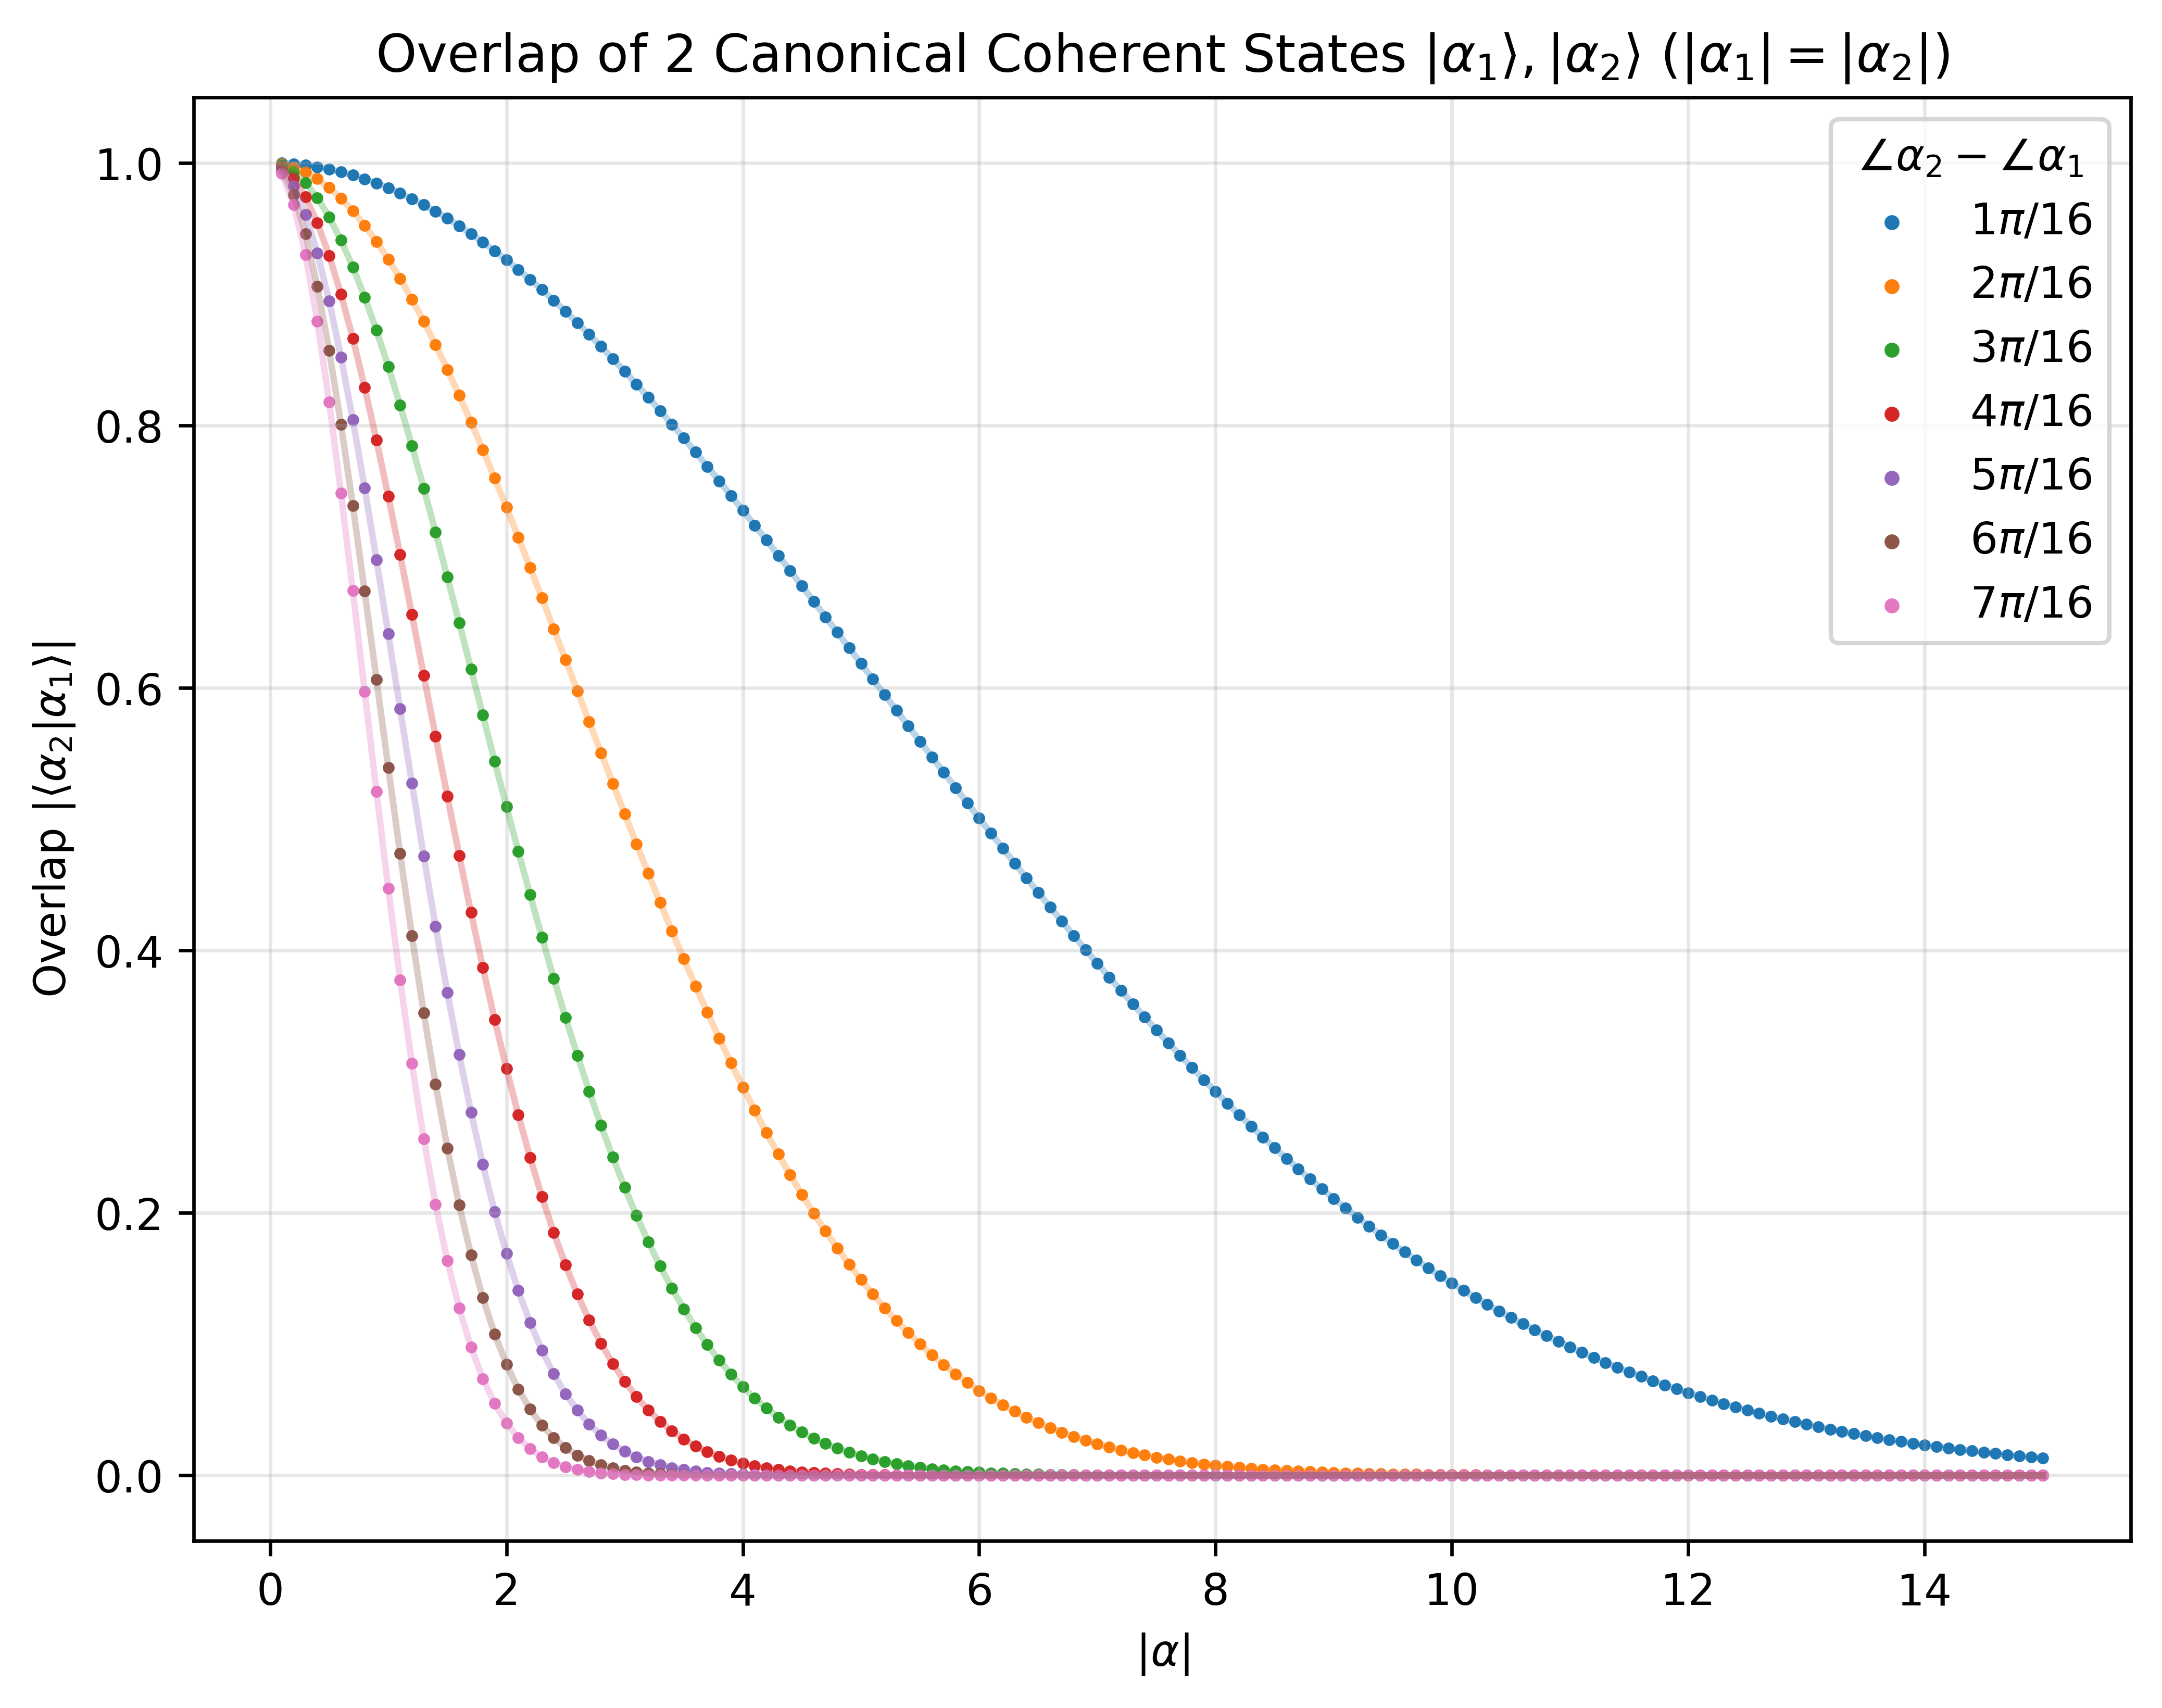
\includegraphics[width=0.7\textwidth]{../figures/overlap.png}
    \end{center}
\end{frame}

\begin{frame}
    \frametitle{Theoretical overlap of canonical coherent states}
    For two different canonical coherent states $\ket{\alpha}$ and $\ket{\beta}$,
    \begin{align}
        \braket{\beta}{\alpha} = e^{-\frac{1}{2}(|\beta|^{2} + |\alpha|^{2} - 2\beta^{*}\alpha)}
    \end{align}

    Assume $\alpha = r_{1}e^{i\theta_{1}}$, $\beta = r_{2}e^{i\theta_{2}}$,
    \begin{align}
        \braket{\beta}{\alpha} = e^{-\frac{1}{2}(r_{1}^{2} + r_{2}^{2} - 2r_{1}r_{2}e^{i(\theta_{1}-\theta_{2})})}
    \end{align}

    If $r_{1} = r_{2} = r$,
    \begin{align}
        \braket{\beta}{\alpha} = e^{-r^{2}(1 - e^{i(\theta_{1}-\theta_{2})})}
    \end{align}

    If $\theta_{1} = \theta_{2} = \theta$,
    \begin{align}
        \braket{\beta}{\alpha} = e^{-\frac{1}{2}(r_{1} - r_{2})^{2}}
    \end{align}
\end{frame}

\subsection{Derivation of MED}

\begin{frame}
    \label{frame:med_math}
    \frametitle{Example (1/4)}
    From Equation \ref{eq:psucc}, the maximal probability happens when $\Pi_{1}$
    projects to the positive eigenspace of
    $p_{1} \ket{\psi_{1}}\bra{\psi_{1}} - p_{2} \ket{\psi_{2}}\bra{\psi_{2}}$.

    For our example,
    \begin{align*}
         & p_{1} \ket{\psi_{1}}\bra{\psi_{1}} - p_{2} \ket{\psi_{2}}\bra{\psi_{2}}
        = 0.5 \times \begin{bmatrix}
                         1 & 0 \\ 0 & 0
                     \end{bmatrix}
        - 0.5 \times \begin{bmatrix}
                         0.5 & 0.5 \\ 0.5 & 0.5
                     \end{bmatrix}                                         \\
         & = 0.5 \times \begin{bmatrix}
                            0.5 & -0.5 \\ -0.5 & -0.5
                        \end{bmatrix}
        \equiv 0.5 A
    \end{align*}
\end{frame}

\begin{frame}
    \frametitle{Example (2/4)}
    The eigenvectors $v_{1}, v_{2}$ and eigenvalues $\lambda_{1}, \lambda_{2}$ of $A$ are
    \begin{align}
         & v_{1} = \begin{bmatrix} -1 - \sqrt{2} & 1   \end{bmatrix} ^{T},
        \lambda_{1} =\frac{\sqrt{2}}{2}                                     \\
         & v_{2} = \begin{bmatrix}  -1 + \sqrt{2} & 1   \end{bmatrix} ^{T},
        \lambda_{2} =\frac{-\sqrt{2}}{2}
    \end{align}

    We choose $v_{1}$ since we want the one with positive eigenvalue.
\end{frame}

\begin{frame}
    \frametitle{Example (3/4)}
    The resulting measurement operators are
    \begin{align*}
         & \Pi_{1} = \frac{v_{1}v_{1}^{T}}{(-1 - \sqrt{2})^{2} + 1^{2}}
        = \begin{bmatrix}
              3 + 2\sqrt{2} & -1 - \sqrt{2} \\
              -1 - \sqrt{2} & 1
          \end{bmatrix}
        / (4 + 2\sqrt{2})                                               \\
         & = (2 - \sqrt{2})\begin{bmatrix}
                               3 + 2\sqrt{2} & -1 - \sqrt{2} \\
                               -1 - \sqrt{2} & 1
                           \end{bmatrix}
        / 4                                                             \\
         & = \begin{bmatrix}
                 (2 + \sqrt{2})/4 & - \sqrt{2}/4     \\
                 - \sqrt{2}/4     & (2 - \sqrt{2})/4
             \end{bmatrix}                        \\
         & \Pi_{2} = I - \Pi_{1} = \begin{bmatrix}
                                       (2 - \sqrt{2})/4 & \sqrt{2}/4       \\
                                       \sqrt{2}/4       & (2 + \sqrt{2})/4
                                   \end{bmatrix}
    \end{align*}
\end{frame}

\begin{frame}
    \frametitle{Example (4/4)}
    The probability of success for MED is
    \begin{align}
         & P_{succ} = p_{1} \bra{\psi_{1}} \Pi_{1} \ket{\psi_{1}}
        + p_{2} \bra{\psi_{2}} \Pi_{2} \ket{\psi_{2}}                  \\
         & = 0.5 \times (2 + \sqrt{2})/4 + 0.5 \times (2 + \sqrt{2})/4 \\
         & = (2 + \sqrt{2})/4 = 0.85355\dots > 0.75
    \end{align}
    (Return to Frame \ref{frame:med_return})
\end{frame}

\begin{frame}[allowframebreaks]{References}
    \bibliography{../back/references, ../back/frio, ../back/uqsd, ../back/attacks}
\end{frame}

\end{document}